\documentclass[12pt,a4paper]{report}

\usepackage{setspace}
\renewcommand{\baselinestretch}{1.2}

\usepackage[round]{natbib}
\usepackage{epsfig}
\usepackage{amsmath,amsfonts,amsthm,amssymb}
\usepackage{setspace}
\usepackage{fancyhdr}
\usepackage{lastpage}
\usepackage{extramarks}
\usepackage{chngpage}
\usepackage{soul}
\usepackage[top=1in, bottom=1in, right=1in, left=1.5in]{geometry}
\usepackage{enumerate}
\usepackage[usenames,dvipsnames]{color}
\usepackage{graphicx,float,wrapfig}
\usepackage{ifthen}
\usepackage{courier}
\usepackage{listings}

\DeclareMathOperator*{\argmin}{\arg\!\min}
\renewcommand\bibname{References}
\definecolor{MyDarkGreen}{rgb}{0.0,0.4,0.0}

\lstloadlanguages{R}%
\lstset{
    language=R,
    frame=single,
    basicstyle=\small\ttfamily,
    keywordstyle=[1]\color{Blue}\bf,
    keywordstyle=[2]\color{Purple},
    keywordstyle=[3]\color{Blue}\underbar,
    identifierstyle=,
    commentstyle=\usefont{T1}{pcr}{m}{sl}\color{MyDarkGreen}\small,
    stringstyle=\color{Purple},
    showstringspaces=false,
    tabsize=5,
    % Put standard R functions not included in the default
    % language here
    morekeywords={rq, qplot, geom, abline, show, guide, aes, brq, lqm, TRUE, FALSE, bayesQR},
    % Put R function parameters here
    morekeywords=[2]{on, off, interp},
    % Put user defined functions here
    morekeywords=[3]{FindESS},
    morecomment=[l][\color{Blue}]{...},
    numbers=left,
    firstnumber=1,
    numberstyle=\tiny\color{Blue},
    stepnumber=5
}

\begin{document}
\begin{titlepage}
\vspace*{\fill}
\begin{center}
\Huge{\textbf{Quantile Regression}}\\
\Large{Reference range of Thyroid function test in pregnancy}\\
\vspace{5mm}
\Large{\textbf{Kevin Brosnan}}\\
\vspace{5mm}
\Large{Final Year Project}\\
\Large{Mathematical Sciences}\\
\vspace{5mm}
\begin{figure}[h]
\begin{center}

\includegraphics{ullogo.jpg}
\end{center}
\end{figure}
\Large{Department Of Mathematics and Statistics}\\
\Large{University of Limerick}\\
\Large{Limerick}\\
\Large{Ireland}\\
\Large{March, 2014}\\
\vspace{10mm}
\large{A final year project submitted in partial fulfillment of the B.Sc degree in Mathematical Sciences}\\
\vspace{6mm}
\Large{Supervisor: Dr. Kevin Hayes}\\
\Large{Second Reader: Dr. Norma Bargary}
\end{center}
\vspace*{\fill}
\end{titlepage}

\pagenumbering{roman}

\chapter*{Abstract}
The aim of this project is to develop a method to provide precise reference ranges for thyroid hormones in women during pregnancy. While other methods have been used in the past, the focus of this research will be to develop these reference ranges using quantile regression. Quantile regression moves away from the general tendency of central regression and is computed at any percentile of interest. Current quantile regression methods do not routinely quantify the precision of the end points of these reference ranges due to a phenomenon called quantile crossing. This results in misclassification of patients to ranges and makes selection for treatment difficult.
\vspace{2mm}

\par\noindent
Thyroid disease is the most common endocrine condition in women of childbearing age and complicates approximately $1\%$ of pregnancies. Physiological changes of pregnancy mean that thyroid hormone reference ranges for non-pregnant women may not be appropriate in pregnancy. The $2.5\%$ and $97.5\%$ regression quantiles will be of interest in this project, as these are the treatment regions for thyroid disease.

\chapter*{Acknowledgements}
I wish to thank the academic staff of the Maths and Statistics Department of University of Limerick for all the knowledge they have instilled on me over the course of my undergraduate programme. I would like to express my deep gratitude to Dr. Kevin Hayes, my supervisor, for his patient guidance, enthusiastic encouragement and useful critiques of my final year project.
\vspace{2mm}
\par\noindent
Finally, I wish to thank my parents for their support and encouragement throughout my study.

\tableofcontents

\clearpage
\pagenumbering{arabic}

\chapter{Introduction}
In statistical regression, the desired estimate of $y|x$ is not always given by a conditional mean, although it is the most commonly used method. While the conditional mean is useful in measuring the relationship between variables around the center of the data, it is often required to understand the relationship between variables at positions other than the center of the data. Quantile regression serves as a method which provides the capabilities to understand the relationship between variables at a given quantile. Throughout this project quantile regression will be used to solely to develop reference ranges for thyroid function in pregnancy, however quantile regression methods have other uses across industry:
\begin{itemize}
    \item A device manufacturer may wish to know what the $5\%$ and $95\%$ quantiles are for some feature of the production process, so as to keep the process under control for $95\%$ of the devices produced
    \item A pediatrician requires a growth chart for children given their age and perhaps even medical back-ground, to help determine whether medical interventions are required
\end{itemize}
Thyroid disorders are the second most common endocrinologic disorders found in pregnancy. Overt hypothyroidism is estimated to occur in $0.3-0.5\%$ of pregnancies. Subclinical hypothyroidism tends to occur in $2-3\%$, and hyperthyroidism is present in $0.1-0.4\%$ \citep{Thyroid-Facts}. Physiological changes of pregnancy, including $50\%$ increase in plasma volume, increased thyroid binding globulin production and a relative iodine deficiency, means that thyroid hormone reference ranges for non-pregnant women may not be appropriate in pregnancy.
\vspace{2mm}

One acceptable approach for establishing legitimate reference ranges requires that a Box-Cox transformation be applied to the data and prediction ranges calculated using classical polynomial regression. Alternatively, non-parametric smoothing such as quantile regression can be used to estimate the $2.5\%$ and $97.5\%$ percentiles. While this approach provides an estimate of the reference range, there are problems with the method. The main problem is the issue of crossing quantiles which makes it difficult to assign each patient to a single range. This is the issue that will be focused on throughout this project.
\vspace{2mm}

Initially a background on quantile regression will be explored. This section will look at the theory behind quantile regression, its advantages and disadvantages over more popular regression methods such as ordinary least squares (OLS) and the implementation of quantile regression under a frequentist approach, a Bayesian approach and a linear mixed effects model approach. Current statistical software based in {\small{\verb"R"}} \citep{R} will be detailed and examined using a sample dataset based on the relationship between household income and food expenditure for working class households in Belgium. The output and computational effort will be provided for comparison between each of the three methods.
\vspace{2mm}

After introducing the key concepts of quantile regression methods, the thyroid data to be modelled in this project will be examined in detail. Descriptive statistics of each of the variables will be provided, along with selection of the principal variables of interest on which the models will be based. The variables will be tested for normality and power transformations provided if necessary to normalise the data. Simple linear quantile models will initially be applied to model the relationship between each of the thyroid hormone variables and the gestation week of the patient. If the simple model does not fit the data to sufficient standard modifications to the model will be made to increase the model fit.
\vspace{2mm}

In the final chapter of this project a solution to the issue of crossing quantile curves will be provided. The theoretical details of the solution will be discussed extensively. The solution to the crossing quantiles will then be applied to model the thyroid hormones once again using the most appropriate model already decided in the exploratory stage. The references ranges for thyroid test function during pregnancy will then be provided using this new approach to non-crossing quantile curve estimation.

\chapter{Analytical Background}\label{Background}
The objective of regression analysis is to establish a relationship between a response variable, $Y$, and the predictor variables, $\{x_{1},\ldots,x_{p}\}$. In real world applications, $Y$ cannot be calculated perfectly from the $X$ variables. For modelling purposes we formulate $Y$, for a fixed value of each $x_{i}$ as a random variable. We generally proceed by summarising the relationship of the response variable for fixed values of the predictors using measures of centrality, specifically the mean, median and mode.
\vspace{2mm}

Quantile regression uses the median as its central tendency and is the method of interest in this project. In this chapter we outline the theory behind quantile regression, focusing attention on the frequentist approach to quantile regression, Bayesian quantile regression and linear quantiles for mixed models. Finally, we will examine the computational implementation required for each of the quantile regression methods outlined above.

\section{Quantiles}
A quantile $\tau$ of the dependant variable $Y$ is defined such that $100\tau\%$ of the population have values less than the $\tau^{th}$ quantile and $100(1-\tau)\%$ of the population have values greater than the $\tau^{th}$ quantile (see Figure \ref{Graph:Quantile}).
\vspace{2mm}

\begin{figure}[ht]\centering
    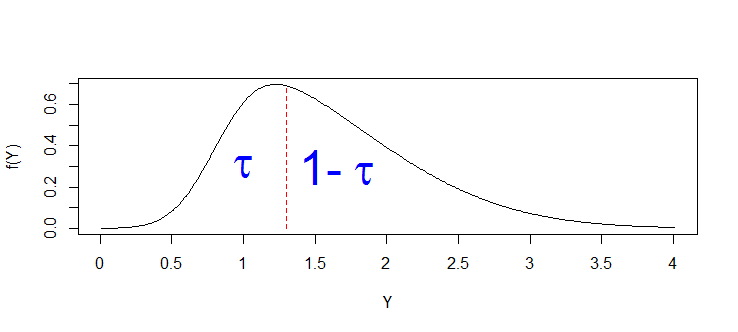
\includegraphics[width=10cm]{Quantiles.png}
    \caption{Graphical illustration of the $\tau^{th}$ quantile.}
    \label{Graph:Quantile}
\end{figure}

The median is defined such that 50\% of your population have a value above this value and 50\% of your population have a value below this value. The median can therefore be interrupted as the $0.5^{th}$ quantile. The quantile or percentile refers to the general case of this.
\vspace{2mm}

More formally, let $Y$ be a continuous real valued random variable, it may be characterised by its distribution function as
    $$F_{Y}(y)=\mathbb{P}(Y \leq y),$$
while for any $0 < \tau <1$,
    $$ Q(\tau) = \inf\left\{y : F_{Y}(y) \geq \tau\right\}$$
is called the $\tau^{th}$ quantile of $Y$. When estimating quantiles, we want to determine the value of $y$ in the sample data corresponding to a given probability $\tau$. The $\tau^{th}$ quantile in a sample of data refers to the probability of $\tau$ for a value $y$, such that
    $$F_{Y}(y_{\tau})=\tau.$$
Another form of expressing the $\tau^{th}$ quantile mathematically is
    $$y_{\tau}=F^{-1}_{Y}(\tau).$$
$y_{\tau}$ is such that it constitutes the inverse of the function $F_{Y}(\tau)$ for a probability $\tau$.
\vspace{2mm}

If the distribution function $F_{Y}(y)$ is monotonically increasing, quantiles are well defined for every $\tau \in (0,1)$. However, if a distribution function $F_{Y}(y)$ is not strictly monotonically increasing, there are some $\tau$'s for which a unique quantile can not be defined. In the latter case one must use the smallest value that $y$ can take on for a given probability $\tau$. In both cases the problem can be defined mathematically as seeking the value of $y$ satisfying
\begin{equation}
\label{eq:Quantiles}
    y_{\tau}=F^{-1}_{Y}(\tau)=\inf\left\{y:F_{Y}(y)\geq\tau\right\}.
\end{equation}
\vspace{2mm}
Therefore, $y_{\tau}$ is equal to the inverse of the function $F_{Y}(\tau)$ which in turn is equal to the infimum of $y$ such that the distribution function $F_{Y}(y)$ is greater or equal to a given probability $\tau$ which in turn is the $\tau^{th}$ quantile.

\section{Quantile Regression}
Quantile regression is a statistical technique used to estimate conditional quantile functions. Classic linear regression methods are based on minimising sum-of-squares residuals and can be used to estimate models for conditional mean functions. Quantile regression methods however offer a way of estimating models for the conditional median function and all other conditional quantile functions. As quantile regression can estimate the entire family of
conditional quantile functions it provides a much more powerful statistical analysis of relationships among random variables \citep{QR-Intro}. The need for something beyond linear regression was first advocated by \citet{Motivation}:
\vspace{2mm}

\par \noindent
{\textit{What the regression curve does is give a grand summary for the averages of the distributions corresponding to the set of x's. We could go further and compute several different regression curves corresponding to the various percentage points of the distributions and thus get a more complete picture of the set. Ordinarily this is not done, and so regression often gives a rather incomplete picture. Just as the mean gives an incomplete picture of a single distribution, so the regression curve gives a correspondingly incomplete picture for a set of distributions.} \citep{Motivation}}
\vspace{2mm}

\begin{flushleft}
Features that characterise quantile regression and distinguish it from other regression methods are the following:
\end{flushleft}
\begin{enumerate}
    \item quantile regression can characterise the entire conditional distribution of $Y$ through different values of $\tau$;
    \item heteroscedasticity can be detected;
    \item median regression estimators can be more efficient then mean regression estimators if heteroscedasticity is detected;
    \item the minimisation problem as illustrated in equation \ref{eq:QR-min} can be solved efficiently by linear programming methods, making estimation easy;
    \item quantiles are robust in regards to outliers.
\end{enumerate}

The technical details in the remainder of this section will help to explain how to implement quantile regression contrasting three fitting methods. Quantile regression can be seen as one statistical method which can be used to complete the regression picture.

\subsection{Frequentist Approach}\label{Background:FA}
Quantile regression transforms a conditional distribution function into a conditional quantile function by slicing it in to segments. These segments describe the cumulative distribution of a conditional variable $Y$ given the explanatory variables $x_{i}$ with the use of quantiles as defined in equation (\ref{eq:Quantiles}). For a dependant variable $Y$ given the explanatory variable $X=x$ and fixed $\tau$, $0<\tau<1$, the conditional quantile function is defined as the $\tau^{th}$ quantile $Q_{Y|X}(\tau|x)$ of the conditional distribution function $F_{Y|X}(y|x)$. For the estimation of the location of the conditional distribution function, the conditional median $Q_{Y|X}(0.5|x)$ can be used as an alternative to the conditional mean.
\vspace{2mm}

In ordinary least squares, modelling a conditional distribution function of a random sample $(y_{1},\ldots,y_{n})$ with a parametric function $\mu(x_{i},\beta)$ where $x_{i}$ represents the independent variables, $\beta$ the corresponding estimates and $\mu$ the conditional mean, one addresses the minimisation problem
    $$\min_{\beta\in\Re}\sum^{n}_{i=1}(y_{i}-\mu(x_{i},\beta))^{2}.$$
We therefore obtain the conditional expectation function $\mathbb{E}[Y|x_{i}]$. The conditional expectation function is the best predictor of $Y$ given $x_{i}$ in the sense that it solves a minimum mean squared error prediction problem. It can be simply evaluated as
$$ \mathbb{E}[Y|x_{i}]=\argmin_{m(x_{i})}\mathbb{E}[(Y-m(x_{i}))^2] $$
where $m(x_{i})$ is any function of $x_{i}$. This equation is minimised at $m(x_{i}) = \mathbb{E}[Y|x_{i}]$. While the approach is similar for quantile regression the central feature now becomes $\rho_{\tau}$, which acts as a check function. Define $\rho_{\tau}(x)$ by
    \[
        \rho_{\tau}(x)=
        \begin{cases}
        \tau*x,& \text{if } x\geq0\\
        (\tau-1)*x,& \text{if } x<0
        \end{cases}
    \]

\begin{figure}[ht]\centering
    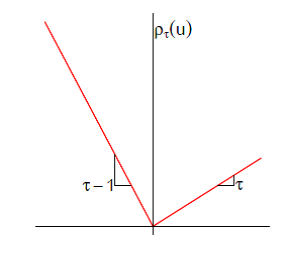
\includegraphics[width=7cm]{CheckFunctionImage.png}
    \caption{Quantile Regression $\rho$ Function}
\end{figure}
\vspace{2mm}

The check function, $\rho_{\tau}(x)$, ensures that:
\begin{enumerate}[(i)]
    \item all $\rho_{\tau}$ are positive;
    \item the scale is according to the probability $\tau$.
\end{enumerate}

In quantile regression, the $\tau^{th}$ \textit{sample} quantile may be found by solving:
\begin{equation}
\label{eq:QR-min}
    \min_{\xi\in\Re}\sum^{n}_{i=1}\rho_{\tau}(y_{i}-\xi)
\end{equation}
While it is more common to define the sample quantiles in terms of the order statistics, $y_{(1)}\leq y_{(2)} \leq \ldots \leq y_{(n))}$, which results in a sorted arrangement of the original sample. Their formulation as a minimisation problem has the advantage that it yields a natural generalisation of the quantiles to the regression context.
The idea of estimating the unconditional mean is simply
$$ \hat{\mu}=\argmin_{\mu\in\Re}\sum(y_{i}-\mu)^{2}.$$
This estimation can be extended to the estimation of the linear conditional mean function $E(Y|X=x)=x'\beta$ by solving
$$ \hat{\beta}=\argmin_{\beta\in\Re^{p}}\sum(y_{i}-x'\beta)^2.$$
Similarly, the linear conditional quantile function, $Q_{Y}(\tau|X=x)=x_{i}'\beta(\tau)$, can be estimated by solving the minimiser
$$ \hat{\beta}=\argmin_{\beta\in\Re^{p}}\sum\rho_{\tau}(y_{i}-x'\beta).$$
In contrast to ordinary least squares, the minimisation in quantile regression is done for each subset defined by $\rho_{\tau}$. The $\tau^{th}$ quantile is estimated with the parametric function $\xi(x_{i},\beta)$. The requirement for the square in the unconditional mean case is to ensure each calculated term is positive, the check function $\rho_{\tau}$ ensures this in the quantile regression case and so the square of difference is not required.

\subsection{Bayesian Approach}
Unlike the frequentist approach to statistics, the Bayesian approach provides us with the entire posterior distribution of the parameter of interest. Additionally, it allows for uncertainty of a parameter to be taken into account when making a prediction. Irrespective of the true distribution of the data, Bayesian inference for quantile regression produces the likelihood function based on the asymmetric Laplace distribution.
\vspace{2mm}

A random variable $\omega$ follows the asymmetric Laplace distribution if its probability density function is given by
$$ f_{\tau}(\omega; \mu,\sigma) = \frac{\tau(1-\tau)}{\sigma}\exp\left\{-\rho_{\tau}\left(\frac{\omega-\mu}{\sigma}\right)\right\}, $$
where $0<\tau<1$, $\mu$ is the location parameter, $\sigma$ is the scale parameter and $\rho_{\tau}(u)$ is the loss function defined as
    \[
        \rho_{\tau}(x)=
        \begin{cases}
        \tau*x,& \text{if } x\geq0\\
        (\tau-1)*x,& \text{if } x<0,
        \end{cases}
    \]
or in a simpler form,
\begin{equation}
\label{eq:Bay-QR}
\rho_{\tau}(u)=\frac{|u|+(2\tau-1)u}{2}.
\end{equation}
\vspace{2mm}

Using general modelling techniques like ordinary least squares the estimates of the regression parameters $\beta$ are computed by assuming that
\begin{enumerate}[(i)]
    \item conditional on $x$, the random variables $Y_{i}$, are mutually independent with distributions $f(y;\mu_{i})$ specified by the values of $\mu_{i}=E[Y_{i}|x_{i}]$;
    \item for some known link function $g$, $g(u_{i})=x_{i}'\beta$.
\end{enumerate}

However, in this project we are interested in the conditional quantile, $q_{\tau}(y_{i}|x_{i})$, in contrast to the conditional mean, $E[Y_{i}|x_{i}]$. Simple assumptions can be made so that regardless of the distribution of the data it is possible to solve for the quantiles in the framework of the general linear model. Assuming the following makes this possible,
\begin{enumerate}[(i)]
    \item $f(y; \mu_{i})$ is asymmetric Laplace;
    \item $g(\mu_{i})=x_{i}'\beta(\tau)=q_{\tau}(y_{i}|x_{i})$ for any $0<\tau<1$.
\end{enumerate}

An issue with using Bayesian statistics is the requirement of a conjugate prior distribution for quantile regression formulation. While this is generally not known Markov Chain Monte Carlo (MCMC) methods can extract posterior distributions of the unknown parameters which allows the use of any prior distribution. While giving us the marginal and joint posterior distributions of all the unknown parameters, the Bayesian approach, also provides us with a very practical way of including parameter uncertainty in predictive inferences.
Given the observations, $y=(y_{1},\ldots,y_{n})$, the posterior distribution of $\beta$, $\pi(\beta|y)$ is given by
$$\pi(\beta|y) \propto L(y| \beta) p( \beta),$$
where $p(\beta)$ is the prior distribution of $\beta$ and $L(y|\beta)$ is the likelihood function written as
\begin{equation}
\label{eq:Bay-Likelihood}
    L(y|\beta)=\tau^{n}(1-\tau)^{n}\exp\left\{-\sum_{i}\rho_{\tau}(y_{i}-x_{i}'\beta)\right\}
\end{equation}
which is using equation \ref{eq:Bay-QR} with a location parameter $\mu_{i}=x_{i}'\beta$.
\vspace{2mm}

The optimum strategy is to choose $\beta$ such that the resulting joint posterior distribution will be proper. It can be shown that the best choice for the prior of $\beta$ is for it to be improper uniform.

\subsection{Linear Mixed Models Approach}
In statistics it is sometimes necessary to take into account the correlation of observations which belong to the same unit or cluster of the data being analysed. Mixed effects models represent an efficient, flexible and popular way of analysing this complex data. The modelling technique attempts to model and estimate the variability between clusters by using cluster specific random effects. The fact that mixed models can estimate the between cluster variability is a significant advantage over standard modelling techniques as they can provide conditional inferences. In mixed models, both fixed and random effects are assumed to be location-shift effects.
\vspace{2mm}

The general idea of linear mixed models approach for quantile regression came from Marco Geraci and Matteo Bottai's asymmetric Laplace approach. A generalisation of this model was further developed by \citet{lqmm} and is the foundation of the {\small\verb"lqmm R"} package which will be discussed later.
\vspace{2mm}

A continuous random variable $\omega\in\Re$ is said to follow an asymmetric Laplace distribution with parameters $(\mu,\sigma,\tau)$, $\omega\sim AL(\mu,\sigma,\tau)$, if its density can be expressed as
$$ p(\omega|\mu,\sigma,\tau)=\frac{\tau(1-\tau)}{\sigma}\exp\left\{-\frac{1}{\sigma}\rho_{\tau}(\omega-\mu)\right\} $$
\vspace{1.5mm}
where $-\infty<\mu<\infty$ is the location parameter, $\sigma >0$ is the scale parameter, $0<\tau<1$ is the skew parameter and $\rho_{\tau}(\upsilon)$ is
    \[
        \rho_{\tau}(x)=
        \begin{cases}
        \tau*x,& \text{if } x\geq0\\
        (\tau-1)*x,& \text{if } x<0
        \end{cases}
    \]
This is the general loss function which is used in each method of quantile regression described in this chapter. In our case, the parameter $\mu$ is of great interest as this is the $\tau^{th}$ quantile of $\omega$, that is that $Pr(\omega\leq\mu)=\tau$.
\vspace{2mm}

If the random variable $\omega$ is comprised of $n$ independent $\omega_{i}'s$ with common skew ($\tau$) and scale ($\sigma$) parameters and different location ($\mu$), then $\omega_{i}\sim AL(\mu_{i},\sigma,\tau)$ for $i={1,\ldots,n}$. This leads to a simplified expression for $\omega's$ density function
$$p(\omega|\mu,\sigma,\tau)=\sigma_{n}(\tau)\exp\left\{-\frac{1}{\sigma}\rho_{\tau}(\omega-\mu)\right\} $$
where $\sigma_{n}(\tau)=\frac{\tau^{n}(1-\tau)^{n}}{\sigma^{n}}$ and $\rho_{\tau}(y-\mu)=\sum_{i=1}^{n}\rho_{\tau}(\omega_{i}-\mu_{i})$.
\vspace{2mm}

\citet{lqmm} proposed a random-intercepts quantile regression model for longitudinal data using the asymmetric Laplace to model the $\tau^{th}$ conditional quantile of a continuous response variable. In particular, they assumed the following regression function
$$ Q_{y|u}(\tau|x,u)=X\beta^{(\tau)} + u,$$
where $(y,X)$ represents the longitudinal data, $u$ a vector of subject-specific random effects and $Q_{y|u}$ denotes the inverse of the unknown distribution $F_{y|u}$. The $\tau^{th}$ regression quantile of $y|u$ was then estimated under the convenient assumption $y|u\sim AL(X\beta^{(\tau)}+u,\sigma^{(\tau)}, \tau)$, where the $\tau$-dependant parameters $\beta^{(\tau)}$ and $\sigma^{(\tau)}$ have a frequentist interpretation. There exists a link between the $L_{1}$ norm regression problem and the asymmetric Laplace based estimation of the coefficients $\beta^{(\tau)}$ which I will not get into here.

\newpage
\section{Implementation}
As {\small\verb"R"} \citep{R} will be used as the development environment for the solution to this problem, we will review the current packages that implement the above quantile regression methods. The main package available in {\small\verb"R"} for each of the methods described above are outlined in the list below. We will discuss each of these methods in the following pages. Advantages, disadvantages and inadequacies of each of the approaches will be highlighted. Included in the following is output from {\small\verb"R"} using the specified approach to compute the quantiles. The sample data used is the Engel data set which is available with the {\small\verb"quantreg"} package available on CRAN. The data consists of income and food expenditure values for $235$ Belgian working class households.

\begin{itemize}
    \item The frequentist method is available in the {\small\verb"quantreg"} package developed by \citet{R-quantreg}
    \item The Bayesian method is available in the {\small\verb"bayesQR"} package developed by \citet{R-bayesQR}
    \item The linear mixed models method is available in the {\small\verb"lqmm"} package developed by \citet{R-lqmm}
\end{itemize}

\subsection{Frequentist Approach}
The frequentist approach to quantile regression is implemented in {\small\verb"R"} through Roger Koenker's extensive {\small\verb"quantreg"} package. The package is currently in version $5.05$. The package contains an array of functions for calculating regression quantiles, plotting the results, formatting the results table and a multitude of data sets which can be used as test data for the package. The basic fitting routine is used as follows {\small\verb"rq(formula, tau=.5, data, method='br')"}. The function can accept more parameters than shown here however these are the parameters of interest here. The {\small\verb"formula"} argument specifies the model that is desired. In the Engel data example below I fitted a simple bivariate linear model so the formula was simply {\small\verb"foodexp ~ income"}, if we had two explanatory variables it would simply be {\small\verb"foodexp~income + something else"}. The parameter {\small\verb"tau"} is defaulted to calculate the median regression line, however it will accept a single quantile of interest or a vector of quantiles which is used in the example below. The {\small\verb"data"} argument requires the name of the {\small\verb"data.frame"} which contains the variables named in the {\small\verb"formula"} argument. In the case of our example {\small\verb"data=engel"} was passed to the function. The {\small\verb"method"} argument specifies the calculation method which the package should use to calculate the regression quantiles of interest.
\vspace{2mm}

The {\small\verb"rq"} function will automatically use {\small\verb"method='br'"} if no method is specified. The {\small\verb"br"} method calculates the regression quantiles using exterior point methods. It controls the quantile regression fitting by the simplex approach embodied in the algorithm of \citet{KdO1987} based on the median regression algorithm of \citet{BR1974}. If all values of {\small\verb"tau"} lie in $(0,1)$ then the regression values are returned for the single or multiple quantiles requested. On the other hand, if {\small\verb"tau"} lies outside $[0,1]$ parametric programming methods are used to find all the solutions to the quantile regression problem for {\small\verb"tau"} in $(0,1)$. This method is efficient for problems containing up to several thousand observations and has the advantage of being able to calculate the full quantile regression process. It also implements a scheme for computing confidence intervals for the estimated parameters based on an inversion of a rank test described in \citet{RK1994}.
\vspace{2mm}

Two other methods to compute the regression quantiles are {\small\verb"method='fn'"} and {\small\verb"method='pfn'"}. These methods both use the Frisch-Newton algorithm to compute the regression quantiles. The algorithms full detail's are explained in \citet{Frisch-Newton}. In brief, the approach is the reverse of the simplex method, rather than travelling around the exterior of the constraint set it starts from within the constraint set and moves towards the exterior. Instead of taking steepest decent steps at each intersection of exterior edges, it takes Newton steps based on a log-barrier Lagrangian form of the objective function. For exceptionally large problems {\small\verb"method='pfn'"} further adds a pre-processing step to the algorithm which can help to speed up the process considerably.
\vspace{2mm}

There are also two methods for penalised quantile regression available in the package are {\small\verb"method='lasso'"} and {\small\verb"method='scad'"}. These methods implement the lasso penalty and Fan and Li's smoothly clipped absolute deviation penalty, respectively. A parameter {\small\verb"lambda"} is passed to both functions and is key to the calculations made. In the {\small\verb"lasso"} case, if {\small\verb"lambda"} is a scalar quantity the penalty function is the l1 norm of the last coefficients, under the assumption that the first coefficient is an intercept parameter that should not be subject to the penalty. When {\small\verb"lambda"} is a vector it defines a coordinatewise specific vector of lasso penalty parameters. Similarly, for the {\small\verb"scad"} method, if {\small\verb"lambda"} is a scalar quantity the penalty function is the scad modified l1 norm of the last coefficients, under the assumption that the first coefficient is an intercept parameter that should not be subject to the penalty. When {\small\verb"lambda"} is a vector it defines a coordinatewise specific vector of scad penalty parameters. It should be noted that while these methods are available, Koenker himself states that ``These methods should probably be regarded as experimental".
\vspace{2mm}

% Plot of Engel data with Quantile lines
\begin{figure}[ht]\centering
    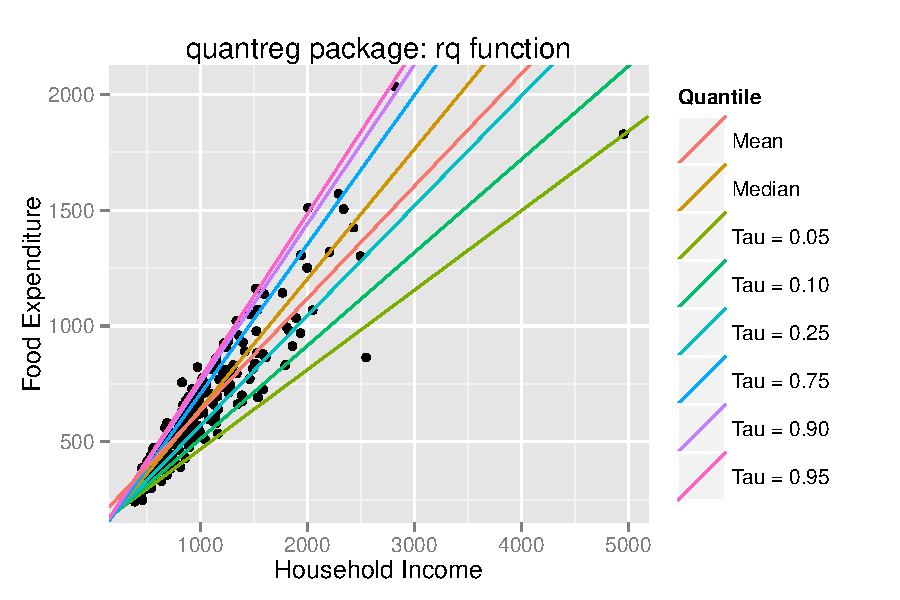
\includegraphics[width=10cm, height=7cm]{PlotofQuantreg.pdf}
    \caption{Quantreg Estimation of Quantiles on Engel Data}
    \label{plot:quantreg-example}
\end{figure}

To provide a somewhat more visual explanation of the {\small\verb"quantreg"} package I will illustrate an example of its usage on the Engel data set available with the package. The data contains $235$ observations of food expenditure and household income for $19^{th}$ century working class Belgian households. Figure \ref{plot:quantreg-example} shows the $\{0.05_{th},0.10_{th},0.25_{th},0.75_{th},0.90_{th},0.95_{th}\}$ quantile regression lines, the median fit and the least squares estimate of the conditional mean function. The quantiles were calculated using the {\small\verb"br"} method as described above. The least squares estimate was computed using the {\small\verb"lm"} function available in {\small\verb"R"} for linear regression. It can be seen at the bottom left of the graph the regression lines intersect with one another which is the issue I hope to address in this paper.
\vspace{2mm}

% Table of Results
\begin{table}[ht]
\begin{center}
\begin{tabular}{|l||c|c|} \hline
\multicolumn{1}{|l||}{Quantile}&\multicolumn{1}{c|}{Intercept}&\multicolumn{1}{c|}{Slope}\tabularnewline
\hline
$\tau$ = 0.05&$\underset{(~98.302,130.517)}{124.880}$&$\underset{(~~0.343,~~0.390)}{~~0.343}$\tabularnewline
$\tau$ = 0.10&$\underset{(~79.888,146.189)}{110.142}$&$\underset{(~~0.342,~~0.451)}{~~0.402}$\tabularnewline
$\tau$ = 0.25&$\underset{(~73.786,120.098)}{~95.484}$&$\underset{(~~0.420,~~0.494)}{~~0.474}$\tabularnewline
Median&$\underset{(~53.259,114.012)}{~81.482}$&$\underset{(~~0.487,~~0.602)}{~~0.560}$\tabularnewline
$\tau$ = 0.75&$\underset{(~32.745,107.314)}{~62.397}$&$\underset{(~~0.580,~~0.690)}{~~0.644}$\tabularnewline
$\tau$ = 0.90&$\underset{(~37.118,103.174)}{~67.351}$&$\underset{(~~0.649,~~0.742)}{~~0.686}$\tabularnewline
$\tau$ = 0.95&$\underset{(~46.265,~83.579)}{~64.104}$&$\underset{(~~0.674,~~0.734)}{~~0.709}$\tabularnewline
Mean&$147.4754$&$~~0.4852$\tabularnewline
\hline
\end{tabular}
\end{center}
\caption{Regression line coefficients for figure \ref{plot:quantreg-example}}
\label{table:quantreg-example}
\end{table}

The quantiles were also calculated after taking a log transformation of the data. This was used as an attempt to stop the quantiles crossing. It can be seen in figure \ref{plot:quantreglog-example} that the quantiles are not crossing at a point close to the origin, however the $0.95^{th}$ and $0.90^{th}$ quantile lines are still crossing. A log transformation therefore does not appear to solve the crossing quantiles problem but does improve on the previous example. The {\small\verb"R"} code used to produce this graphic is available in appendix \ref{App:Engel-Code-Quantreg}.

% Plot of log of Engel data with Quantile lines
\begin{figure}[ht]\centering
    \includegraphics[width=10cm]{PlotofQuantregLog.pdf}
    \caption{Quantreg Estimation of Quantiles on log transformation of Engel Data}
    \label{plot:quantreglog-example}
\end{figure}

Finally, the coefficients of the quantile regression calculations for figure \ref{plot:quantreg-example} are shown in table \ref{table:quantreg-example} while the log transformation coefficients are shown in table \ref{table:quantreglog-example}. The values in parenthesis below the actual value are the confidence bands for that value. Note that the intercept and the slope differ for each of the quantiles and the linear regression model.
\vspace{2mm}

% Table of log Results
\begin{table}[ht]
\begin{center}
\begin{tabular}{|l||c|c|} \hline
\multicolumn{1}{|l||}{Quantile}&\multicolumn{1}{c|}{Intercept}&\multicolumn{1}{c|}{Slope}\tabularnewline
\hline
$\tau$ = 0.05&$\underset{(0.2283,0.4607)}{0.2638}$&$\underset{(0.7398,0.8213)}{0.8113}$\tabularnewline
$\tau$ = 0.10&$\underset{(0.1130,0.3601)}{0.3033}$&$\underset{(0.7866,0.8645)}{0.8041}$\tabularnewline
$\tau$ = 0.25&$\underset{(0.1249,0.4095)}{0.2151}$&$\underset{(0.7822,0.8799)}{0.8495}$\tabularnewline
Median&$\underset{(0.0303,0.3911)}{0.1817}$&$\underset{(0.8051,0.9302)}{0.8766}$\tabularnewline
$\tau$ = 0.75&$\underset{(-0.0057,0.2805)}{0.1048}$&$\underset{(0.8552,0.9535)}{0.9156}$\tabularnewline
$\tau$ = 0.90&$\underset{(0.0335,0.2759)}{0.2075}$&$\underset{(0.8674,0.9493)}{0.8909}$\tabularnewline
$\tau$ = 0.95&$\underset{(0.0804,0.2771)}{0.1258}$&$\underset{(0.8720,0.9381)}{0.9222}$\tabularnewline
Mean&$0.2368$&$0.8559$\tabularnewline
\hline
\end{tabular}
\end{center}
\caption{Regression line coefficients for figure \ref{plot:quantreglog-example}}
\label{table:quantreglog-example}
\end{table}

\subsection{Bayesian Approach}
The implementation of the Bayesian approach to quantile regression is available in the {\small\verb"bayesQR"} package developed by \Citeauthor{R-bayesQR}. The implementation as expected is much less efficient with regard to processing time than the {\small\verb"quantreg"} package due to the iteration process required for Bayesian calculations. The package currently resides in version $2.1$ and was updated in $2013$. The quantile regression function is called by {\small\verb"bayesQR(formula, data, quantile=0.5, ndraw, prior)"}.
\vspace{2mm}

The {\small\verb"formula"} argument specifies the model that is desired. It follows the same format as in the {\small\verb"rq"} function discussed earlier. The {\small\verb"data"} parameter is an optional parameter to specify the data object from which the dependant and independent variables are taken. The parameter {\small\verb"quantile"} is defaulted to calculate the median regression line, however it will accept a single quantile of interest and will also accept a vector of quantiles as was an option in the {\small\verb"quantreg"} package. The {\small\verb"ndraw"} parameter specifies how many Markov Chain Monte Carlo draws are to be taken when estimating each quantile required. The {\small\verb"prior"} argument allows the user to pass a prior distribution to the model if known otherwise the prior distribution is calculated based on the model type being used.
\vspace{2mm}

The package can compute Bayesian quantiles for four types of models; continuous dependant variable without adaptive lasso variable selection, continuous dependant variable with adaptive lasso variable selection, binary dependant variable without adaptive lasso variable selection and binary dependant variable with adaptive lasso variable selection. The computational effort required for each of these methods is similar and is in general extremely computationally intense given a relatively large data set.

% Plot of Engel data with Quantile lines
\begin{figure}[ht]\centering
    \includegraphics[width=10cm,height=7cm]{PlotofBayesQR.pdf}
    \caption{bayesQR Estimation of Quantiles on Engel Data}
    \label{plot:bayesQR-example}
\end{figure}

Figure \ref{plot:bayesQR-example} shows the regression quantiles produced by the {\small\verb"bayesQR"} method on the same data used in the {\small\verb"quantreg"} example above. The regression lines are close but not identical to those produced by the frequentist approach in figure \ref{plot:quantreg-example}. The problem of crossing quantiles is still present when using the Bayesian approach to quantile regression.
\vspace{2mm}

% Table of Results
\begin{table}[ht]
\begin{center}
\begin{tabular}{|l||c|c|} \hline
\multicolumn{1}{|l||}{Quantile}&\multicolumn{1}{c|}{Intercept}&\multicolumn{1}{c|}{Slope}\tabularnewline
\hline
Tau = 0.05 & ~124.561 & 0.344 \tabularnewline
Tau = 0.10 & ~107.495 & 0.403 \tabularnewline
Tau = 0.25 & ~94.078 & 0.475 \tabularnewline
Median & ~81.227 & 0.560 \tabularnewline
Tau = 0.75 & ~57.229 & 0.650 \tabularnewline
Tau = 0.90 & ~64.690 & 0.689 \tabularnewline
Tau = 0.95 & ~64.605 & 0.708 \tabularnewline
Mean & 147.475 & 0.485 \tabularnewline
\hline
\end{tabular}
\end{center}
\caption{Regression line coefficients for figure \ref{plot:bayesQR-example}}
\label{table:bayesQR-example}
\end{table}

As before the quantiles were also calculated after taking a log transformation of the data. It can be seen in figure \ref{plot:bayesQRlog-example} that the quantiles appear not to cross anywhere in the domain in which it is plotted. The {\small\verb"R"} code used for the two graphics can be found in appendix \ref{App:Engel-Code-bayesQR}.

% Plot of log transformation of Engel data with Quantile lines
\begin{figure}[ht]\centering
    \includegraphics[width=10cm,height=7cm]{PlotofBayesQRLog.pdf}
    \caption{bayesQR Estimation of Quantiles on log transformation of Engel Data}
    \label{plot:bayesQRlog-example}
\end{figure}


Finally, the coefficients of the quantile regression calculations for figure \ref{plot:bayesQR-example} are shown in table \ref{table:bayesQR-example} while the log transformation coefficients are shown in table \ref{table:bayesQRlog-example}. The {\small\verb"bayesQR"} package does not provide a simple method for computing the confidence intervals for the quantiles. Note that the intercept and the slope differ for each of the quantiles and the linear regression model. The values are also different to those calculated by the {\small\verb"quantreg"} package.
\vspace{2mm}

% Table of log Results
\begin{table}[ht]
\begin{center}
\begin{tabular}{|l||c|c|} \hline
\multicolumn{1}{|l||}{Quantile}&\multicolumn{1}{c|}{Intercept}&\multicolumn{1}{c|}{Slope}\tabularnewline
\hline
Tau = 0.05 & 0.2395 & 0.8084 \tabularnewline
Tau = 0.10 & 0.2194 & 0.8236 \tabularnewline
Tau = 0.25 & 0.1976 & 0.8465 \tabularnewline
Median & 0.2184 & 0.8653 \tabularnewline
Tau = 0.75 & 0.2323 & 0.8798 \tabularnewline
Tau = 0.90 & 0.2312 & 0.8943 \tabularnewline
Tau = 0.95 & 0.2653 & 0.9031 \tabularnewline
Mean & 0.2368 & 0.8559 \tabularnewline
\hline
\end{tabular}
\end{center}
\caption{Regression line coefficients for figure \ref{plot:bayesQRlog-example}}
\label{table:bayesQRlog-example}
\end{table}

\subsection{Linear Mixed Models Approach}
The final package which will be presented here is the {\small\verb"lqmm"} package developed by Marco Geraci. The package is the {\small\verb"R"} implementation of linear mixed models approach for quantile regression. The package is currently in version $1.03$ and was updated in $2013$. The package contains a multitude of functions based around the implementation of the asymmetric Laplace solution to the regression quantiles. The functions of most interest are {\small\verb"lqm"} and {\small\verb"lqmm"} as these are the methods which calculate the regression quantiles.
\vspace{2mm}

The {\small\verb"lqm"} function is called using {\small\verb"lqm(formula, data, iota=0.5)"}. The {\small\verb"formula"} and {\small\verb"data"} arguments are specified exactly as they were in the {\small\verb"quantreg"} packages {\small\verb"rq"} function. The {\small\verb"iota"} parameter is equivalent to the {\small\verb"tau"} parameter in the previous two packages and can accept single or multiple tau values. The function computes an estimate of the $\tau^{th}$ quantile function of the response variable, conditional on the covariates, as specified by the {\small\verb"formula"} argument. The quantile predictor is assumed to be linear. The function maximises the likelihood of a Laplace regression which is equivalent to the minimisation of the weighted sum of absolute residuals. The optimisation algorithm is based on the gradient of the Laplace log-likelihood.
\vspace{2mm}

% Plot of Engel data with Quantile lines
\begin{figure}[ht]\centering
    \includegraphics[width=10cm]{PlotofLqmm.pdf}
    \caption{lqmm Estimation of Quantiles on Engel Data}
    \label{plot:lqmm-example}
\end{figure}

The {\small\verb"lqmm"} function is called using {\small\verb"lqmm(fixed, random, iota=0.5)"}. The function is similar to the {\small\verb"lqm"} function but allows random effects to be specified as arguments. The {\small\verb"fixed"} and {\small\verb"iota"} parameters follow directly from the {\small\verb"formula"} and {\small\verb"iota"} arguments in the {\small\verb"lqm"} function. The {\small\verb"random"} argument allows the inclusion of random effects and should be specified as {\small\verb"~x1+ ... + xn"}, where $x_{i}$ is a random effect of interest. The function calculates an estimate of the $\tau^{th}$ quantile function of the response, conditional on the covariates, as specified by the {\small\verb"fixed"} argument and on random effects, as specified by the {\small\verb"random"} argument. The quantile predictor is again assumed to be linear and the function maximises the likelihood Laplace regression. The likelihood is numerically integrated via Gaussian quadrature techniques. The optimisation algorithm ia based on the gradient of the Laplace log-likelihood.
\vspace{2mm}

% Table of Results
\begin{table}[ht]
\begin{center}
\begin{tabular}{|l||c|c|} \hline
\multicolumn{1}{|l||}{Quantile}&\multicolumn{1}{c|}{Intercept}&\multicolumn{1}{c|}{Slope}\tabularnewline
\hline
$\tau$ = 0.05&147.475&~~0.329\tabularnewline
$\tau$ = 0.10&147.475&~~0.354\tabularnewline
$\tau$ = 0.25&147.475&~~0.417\tabularnewline
Median&147.475&~~0.487\tabularnewline
$\tau$ = 0.75&147.475&~~0.553\tabularnewline
$\tau$ = 0.90&147.476&~~0.613\tabularnewline
$\tau$ = 0.95&147.476&~~0.629\tabularnewline
Mean&147.475&~~0.485\tabularnewline
\hline
\end{tabular}
\end{center}
\caption{Regression line coefficients for figure \ref{plot:lqmm-example}}
\label{table:lqmm-example}
\end{table}

Again, I have used the Engel data set as the example data set to allow comparison between the three packages. I have used the {\small\verb"lqm"} function to calculate the regression quantiles for this example. In figure \ref{plot:lqmm-example} we can see that the regression quantiles appear to meet at a point on the y-axis. However, the median regression line and the mean regression line seem to be identical which is vastly different from what was experienced using the other two packages. The extreme quantile lines, $\tau=\{0.95,0.05\}$, appear much closer to the median regression fit than they did previously.
\vspace{2mm}

% Plot of log transformation of Engel data with Quantile lines
\begin{figure}[ht]\centering
    \includegraphics[width=10cm, height=7cm]{PlotofLqmmLog.pdf}
    \caption{lqmm Estimation of Quantiles on log transformation of Engel Data}
    \label{plot:lqmmlog-example}
\end{figure}

When we look at table \ref{table:lqmm-example}, which contains the coefficients for the graphic in figure \ref{plot:lqmm-example}, we can see that all the intercepts calculated by {\small\verb"lqm"} are exactly equal to the intercept of the least squares estimate for the conditional mean function. This is vastly different from the other two packages where none of the intercepts were equal.
\vspace{2mm}

Finally, a plot of the quantiles calculated by {\small\verb"lqm"} for the data after a log transformation is shown in figure \ref{plot:lqmmlog-example}. Again it seems to help in addressing the issue of crossing quantiles, however the upper quantiles, $0.90^{th}$ and $0.95^{th}$, are again very close which could cause a problem. The coefficients are given in table \ref{table:lqmmlog-example}. The {\small\verb"R"} code required to reproduce the graphics and coefficients shown in this section can be found in appendix \ref{App:Engel-Code-lqmm}.

% Table of log Results
\begin{table}[ht]
\begin{center}
\begin{tabular}{|l||c|c|} \hline
\multicolumn{1}{|l||}{Quantile}&\multicolumn{1}{c|}{Intercept}&\multicolumn{1}{c|}{Slope}\tabularnewline
\hline
$\tau$ = 0.05&0.2259&0.8232\tabularnewline
$\tau$ = 0.10&0.2285&0.8306\tabularnewline
$\tau$ = 0.25&0.2327&0.8438\tabularnewline
Median&0.2372&0.8577\tabularnewline
$\tau$ = 0.75&0.2409&0.8689\tabularnewline
$\tau$ = 0.90&0.2441&0.8780\tabularnewline
$\tau$ = 0.95&0.2452&0.8814\tabularnewline
Mean&0.2368&0.8559\tabularnewline
\hline
\end{tabular}
\end{center}
\caption{Regression line coefficients for figure \ref{plot:lqmmlog-example}}
\label{table:lqmmlog-example}
\end{table}



\chapter{Regression Quantiles for Thyroid Data}\label{ThyroidReg}
The previous chapters in this paper have examined existing quantile regression methods in {\small\verb"R"} using sample datasets. However, the central focus of this research paper is to develop thyroid reference ranges in pregnancy using quantile regression. This chapter will include the following:
\begin{itemize}
    \item introducing the thyroid data which will be used throughout this report;
    \item fitting linear models to the thyroid data using existing {\small\verb"R"} packages;
    \item outlining the inadequacies of current packages for quantile regression.
\end{itemize}

\section{Thyroid Data}
The thyroid data used in this research project was collected from pregnant women who attended a large maternity hospital between February $2010$ and February $2011$. A sample size of $300$ or more women were sought for the analysis as results from \citet{Cotzias2008} had shown amble power from a sample size of $300$ women.
\vspace{2mm}

Healthy women attending the antenatal care clinic with a singleton pregnancy were randomly selected for participation in the study. Women with known thyroid disease, autoimmune diseases, diabetes mellitus, recurrent miscarriage, hyperemesis gravidarum and pre-eclampsia were excluded from the study. The women who took part in the study were between $10$ and $42$ weeks of gestation, and each woman was sampled on only one occasion. Each individual assessed also had an uncomplicated medical history to avoid discrepancies in the results caused by underlying health conditions.
\vspace{2mm}

The final data file consists of $10$ variables, each of which is shown in the data extract below, and samples taken from $311$ pregnant women. The key concern of this project is to develop gestation-specific reference ranges for each of the following thyroid hormones:
\begin{description}
    \item[T4] level of thyroxine hormone in each patient
    \item[T3] level of triiodothyronine hormone in each patient
    \item[TSH] level of thyroid stimulating hormone in each patient
    \item[TPO] level of thyroid peroxidase enzyme in each patient
\end{description}
\vspace{2mm}

The sample dataset available contains data for the $1^{st}$, $2^{nd}$ and $3^{rd}$ trimesters of pregnancy. The $1^{st}$ trimester data was recorded during the $10^{th}-14^{th}$ weeks of gestation, while the $2^{nd}$ and $3^{rd}$ trimesters were recorded in the $14^{th}-26^{th}$ week period of gestation and the $27^{th}-42^{nd}$ week period of gestation respectively.  A sample of the combined dataset can be seen in table \ref{table:sampledata}. A data dictionary for the variables of the thyroid data is given in table \ref{table:sampledatadict}.
\vspace{2mm}
\vspace{2mm}

% Table of Thyroid Final Data
\begin{table}[ht]
\begin{center}
\begin{tabular}{|l|c|c|c|c|c|c|c|c|c|}\hline \multicolumn{1}{|l|}{MRN}&\multicolumn{1}{c|}{Age}&\multicolumn{1}{c|}{Ethnicity}&\multicolumn{1}{c|}{Smoking}&\multicolumn{1}{c|}{T4}&\multicolumn{1}{c|}{TSH}&\multicolumn{1}{c|}{T3}&\multicolumn{1}{c|}{TPO}&\multicolumn{1}{c|}{Gestation}&\multicolumn{1}{c|}{Trimester}\tabularnewline
\hline
~937395 & 30 & Irish & No & 14.6 & 0.37 & 4.6 & 5.3 & 12.00 & T1 \tabularnewline
1975207 & 28 & Irish & No & 13.8 & 2.07 & 5.3 & 0.0 & 13.00 & T1 \tabularnewline
~464433 & 28 & Irish & No & 13.8 & 1.16 & 4.8 & 0.0 & 12.00 & T1 \tabularnewline
1123123 & 28 & Irish & No & 12.3 & 2.71 & 4.7 & 5.2 & 12.00 & T1 \tabularnewline
1855554 & 35 & Irish & No & 14.3 & 0.57 & 4.8 & 0.0 & 13.29 & T1 \tabularnewline
1068450 & 28 & Irish & No & 14.2 & 2.39 & 4.5 & 7.0 & 12.86 & T1 \tabularnewline
2099487 & 26 & Polish & No & 11.0 & 2.82 & 4.8 & 22.9 &22.00 & T2 \tabularnewline
2162414 & 34 & English & No & 14.0 & 0.62 & 4.7 & 6.8 & 14.43 & T2 \tabularnewline
\hline
\end{tabular}
\end{center}
\caption{Extract from Thyroid data}
\label{table:sampledata}
\end{table}

\begin{table}[ht]
\begin{center}
\begin{tabular}{|p{2.5cm}p{10cm}|}\hline
\multicolumn{1}{|c}{\textbf{Variable}}&\multicolumn{1}{c|}{\textbf{Description}}\tabularnewline
\hline\hline
\textbf{MRN}&unique hospital identifier for each patient \tabularnewline
\textbf{Age}&age of patient in years \tabularnewline
\textbf{Ethnicity}&country/region of birth \tabularnewline
\textbf{Smoking}&binomial response yes or no, if yes the number of cigarettes smoked per day is recorded \tabularnewline
\textbf{T4}&level of thyroxine hormone in each patient \tabularnewline
\textbf{TSH}&level of thyroid stimulating hormone in each patient \tabularnewline
\textbf{T3}&level of triiodothyronine hormone in each patient \tabularnewline
\textbf{TPO}&level of thyroid peroxidase enzyme in each patient \tabularnewline
\textbf{Gestation}&number of weeks pregnant \tabularnewline
\hline
\end{tabular}
\end{center}
\caption{Data dictionary for thyroid data}
\label{table:sampledatadict}
\end{table}

\section{Descriptive Statistics}
This section provides descriptive statistics which describe the maternal characteristics of the population in this study. A graphical view of the distribution of each of the $4$ thyroid hormone variables in our dataset is also provided, along with appropriate statistical tests, is also included. If any of the variables of interest exhibited skewness, the Box-Cox method was used to identify the optimal power transformation to achieve normality of the data \citep{BoxCox1964}, a brief explanation of which is provided later.
\vspace{2mm}

The final study population, had a median maternal age of $30$ years, with an interquartile range of $27-33$ years and a range from $17-40$ years. The population could be divide into four key geographical groupings as follows:
\begin{itemize}
    \item {\textbf{White Irish}} $77.5\%$ (n=$241$)
    \item {\textbf{European}} $16.1\%$ (n=$50$)
    \item {\textbf{Asian}} $4.5\%$ (n=$14$)
    \item {\textbf{African}} $1\%$ (n=$3$)
\end{itemize}
\vspace{2mm}

Of the $311$ women in the final study population, over three-quarters of the individuals were non-smokers ($77.8\%$), with only $2.6\%$ of the population smoking more than $10$ cigarettes per day. Finally, the data was split evenly across the trimesters with $34.4\%$ of women tested being in the $1^{st}$ trimester, while $32.8\%$ of the population were tested during both their $2^{nd}$ and $3^{rd}$ trimesters.

\vspace{2mm}

As part of the instal analysis of the data, correlation among each of the thyroid hormone variables were calculated. It was found that a statistically significant relationship existed between TPO and TSH (Pearson's r value $0.230$, p-value $=$ $0.001$). No other correlations among the thyroid hormone variables existed at a statistically significant level. However, due to the relationship between TSH and TPO it was decided to not model on TPO in our analysis. Therefore, the variables of interest are now free T$4$, free T$3$ and TSH.

\subsection{Distributions of variables}
When producing statistical models it is appropriate to model data that is normally distributed. If the initial data is not normally distributed then a power transformation such as a Box-Cox transformation can be applied to the data to correct this. The distributions for each of the four thyroid hormone variables (free T$4$, free T$3$, TSH, TPO) will be examined in this section using quantile-quantile plots (Q-Q plots), histograms and box-plots. A Shapiro-Wilk normality test will also be applied to the data and an interpretation of the results will be detailed.
\vspace{2mm}

\begin{figure}[ht]\centering
    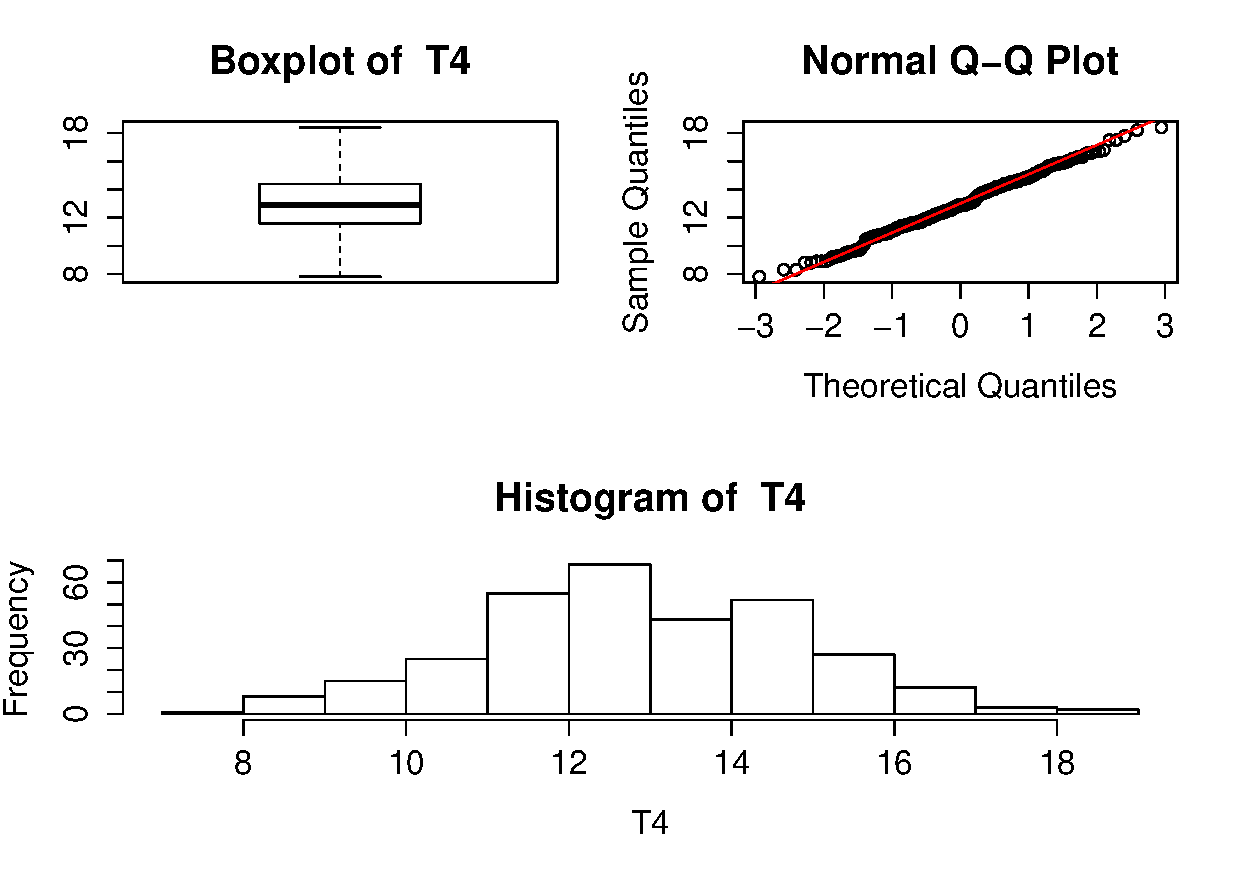
\includegraphics[width=10cm,height=7cm]{NormT4.pdf}
    \caption{Distribution Plots for free T4}
    \label{Distribution:T4}
\end{figure}
\vspace{2mm}

The normality plots for free T$4$ can be seen in figure \ref{Distribution:T4}. The QQ-plot, boxplot and histogram show slightly heavy tails but otherwise it appears that the free T$4$ data is normally distributed. A Shapiro-Wilk test carried out on free T$4$ verified this conclusion further, as a p-value of $0.45$ (Shapiro-Wilk W value $0.9952$), resulting in a failure to reject the null hypothesis that the data is normally distributed. Thus no transformation of the free T$4$ data is required.
\vspace{2mm}

\begin{figure}[ht]\centering
    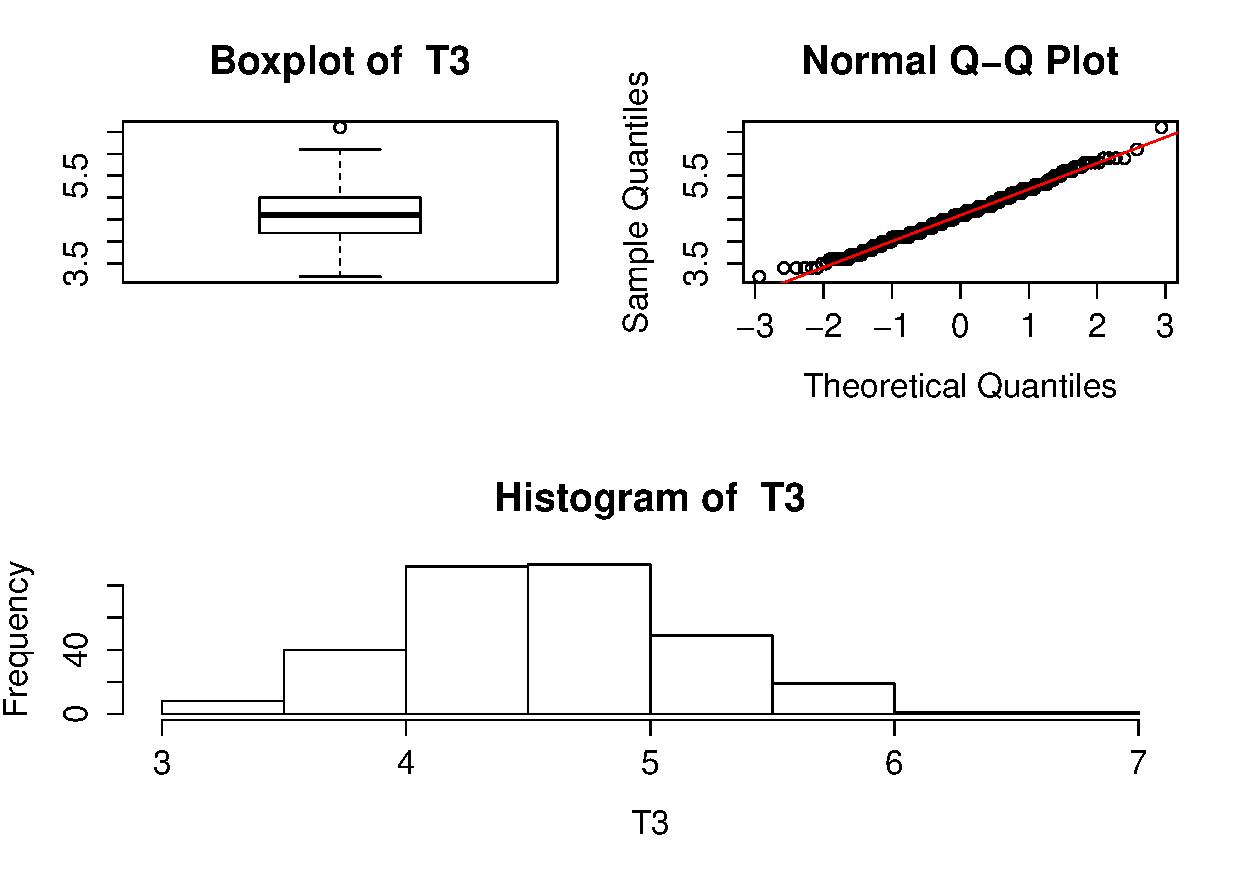
\includegraphics[width=10cm, height=7cm]{NormT3.pdf}
    \caption{Distribution Plots for free T3}
    \label{Distribution:T3}
\end{figure}
\vspace{2mm}

Equivalent to the plots produced for free T$4$ the corresponding plots for free T$3$ can be seen in figure \ref{Distribution:T3}. Similarly to free T$4$ the T$3$ data looks relatively normally distributed in each of the plots produced, with the exception of one outlier in the upper tail of the distribution. Carrying out the Shapiro-Wilk test for normality results in a p-value of $0.13$ (Shapiro-Wilk W value $0.9925$) which is not statistically significant at the $5\%$ level and so again we fail to reject the null hypothesis that the T$3$ data is normally distributed. As before no transformation of the T$3$ data will be required before modelling.
\vspace{2mm}

The normality checks for TSH can be seen in figure \ref{Distribution:TSH}. The boxplot shows two outliers in the upper range of the TSH data. The QQ-plot also shows a departure from normality at each of the tails. From the histogram it can be seen that the data is positively skewed. Carrying out the Shapiro-Wilk  normality test for TSH results in a p-value of $0.0001$ (Shapiro-Wilk W value $0.9784$) which is statistically significant. Therefore, the null hypothesis is rejected in favour of the alternative hypothesis, that the TSH data is not normally distributed. Therefore, a power transform of TSH will be required prior to modelling the regression quantiles for the variable.

\begin{figure}[ht]\centering
    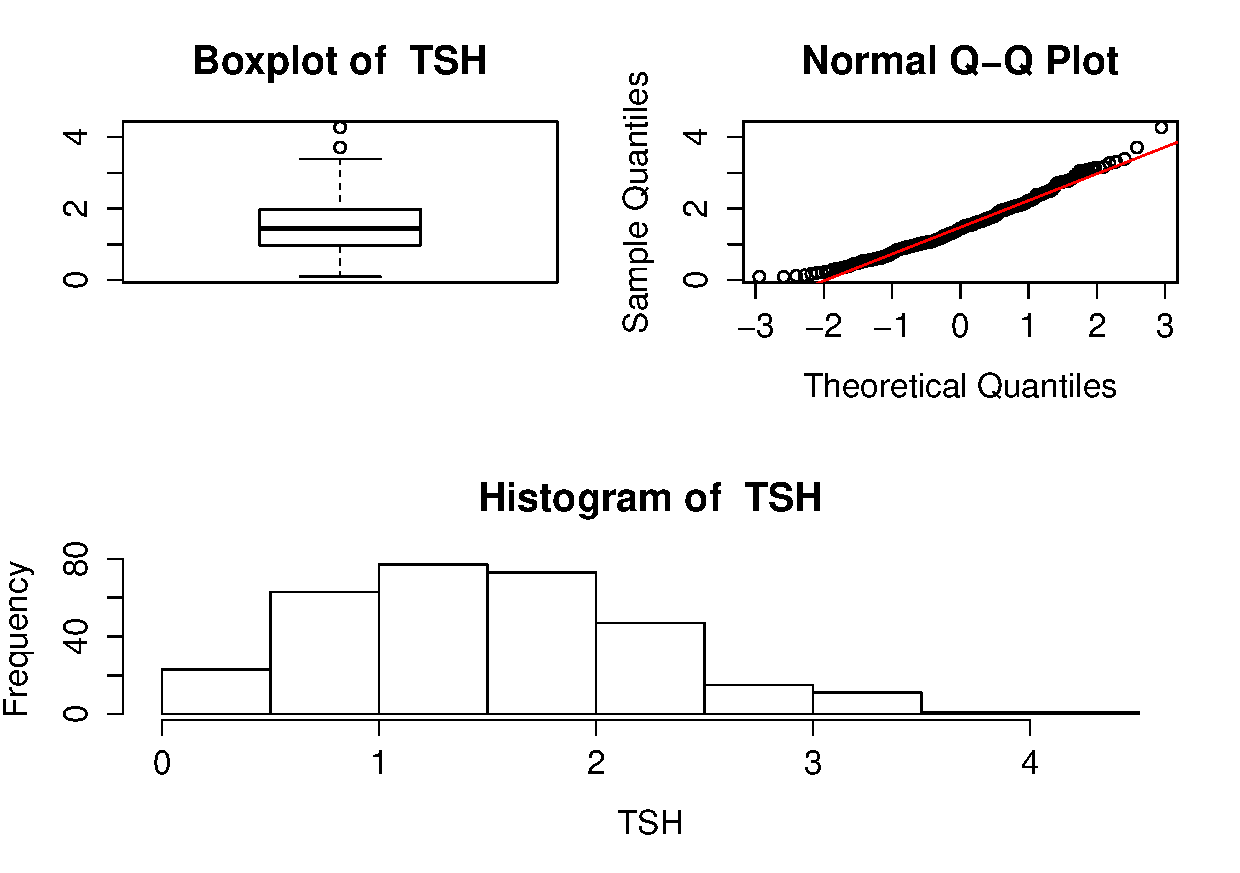
\includegraphics[width=10cm, height=8cm]{NormTSH.pdf}
    \caption{Distribution Plots for TSH}
    \label{Distribution:TSH}
\end{figure}
\vspace{2mm}

All of the {\small\verb"R"} code for the plots and statistics calculated in this section can be found in Appendix \ref{App:Distributions}.

\subsection{Box-Cox Transformation}
In statistical models many important features follow from the assumption that the data being modelled is normally distributed with a common variance and additive error structure \citep{BoxCoxReview}. Once the theoretical assumptions required for the modelling technique are approximately satisfied, then the usual procedures can be applied. In situations where the assumptions are seriously violated several options are available:
\begin{enumerate}
    \item ignore the violation of the assumptions and carry out the modelling procedure as if all assumptions were satisfied
    \item for each of the violated assumptions decide on a more appropriate assumption and use a valid technique that takes account of this new assumption
    \item design a new model that has important aspects of the original model and satisfies all the assumptions - apply a power transformation to the data or remove evident outliers in the data
    \item use a distribution-free procedure that is valid even if various assumptions are violated
\end{enumerate}

In the vast majority of cases $(iii)$ is chosen as the best procedure to follow. In this paper I will use the Box-Cox power transformation for data which is not normally distributed. The Box-Cox transformation is defined as follows

\[
        y_{i}=
        \begin{cases}
        y_{i}^{\lambda},& \text{if } \lambda\neq0\\
        \log(y_{i}),& \text{if } \lambda=0
        \end{cases}
    \]
\vspace{2mm}

From a modelling perspective this results in transforming the data before modelling and then transforming it back to be in line with the original dataset. For a simple linear model of the form
$$y = \alpha + \beta x + \epsilon$$
a power transformation of the $y$ variable results in modelling
\[
    \begin{cases}
    y^{\lambda} = \alpha + \beta x + \epsilon$$, & \text{if } \lambda\neq0\\
    \log(y) = \alpha + \beta x + \epsilon$$, & \text{if } \lambda=0
    \end{cases}
\]
However, this model needs to be transformed back to the original variables which results in the following
\[
    \begin{cases}
    y = (\alpha + \beta x + \epsilon)^{\frac{1}{\lambda}},  & \text{if } \lambda\neq0\\
    y = e^{(\alpha + \beta x + \epsilon)}, & \text{if } \lambda=0
    \end{cases}
\]
\vspace{2mm}

After the instal exploration of the variables of interest in the thyroid data, it was shown that only TSH required a transformation before modelling. Using the {\small\verb"box.cox"} method (see Appendix \ref{App:BoxCox}) it was shown that the optimal value of $\lambda$ was $0.59$. However, a square root transformation ($\lambda=0.5$) is much more practical to use.

\begin{figure}[ht]\centering
    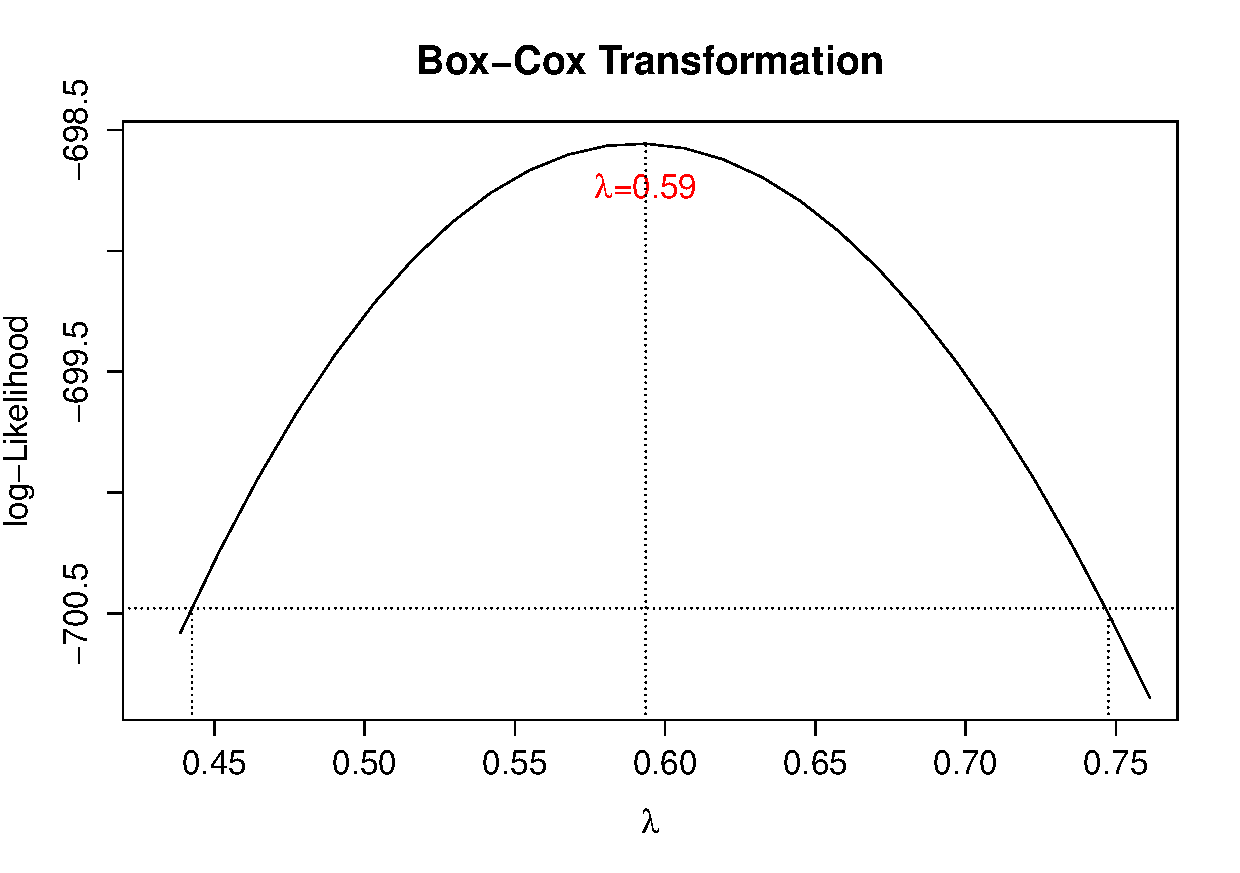
\includegraphics[width=10cm, height=8cm]{BoxCoxTSH.pdf}
    \caption{Box-Cox transformation parameter for TSH}
\end{figure}
\vspace{2mm}


From the above output, the model that will now be used to calculate the regression quantiles for TSH will be
$$ \sqrt{TSH} = \alpha + \beta (Gestation) + \epsilon$$


\section{Linear Quantile Models}
The main objective of this project is to develop a method which can calculate reference ranges for each of the variables with respect to the gestation week. This allows the medical practitioners to gain information on those patients who should be treated for thyroid disease. Quantile regression is the method of choice for calculating the reference ranges, however as has already been discussed in detail the crossing of the quantiles causes problems for classifying patients for treatment or not.
\vspace{2mm}

In this section, the quantile regression models will be developed for each of our thyroid hormone variables (T$4$, T$3$, TSH). Each will be modelled with respect to gestation week of the patient, in a hope to develop reference ranges for thyroid disease during pregnancy. This issue of crossing quantiles will be addressed in the next chapter and so observations of such behaviour will be mentioned here but not expanded upon.
\vspace{2mm}

The {\small{\verb"R"}} code required for producing the quantile models and the graphics in this section can be found in Appendix \ref{App:QuantileModelsT3}.

\subsection{Free T4}
As stated earlier in this chapter the free T$4$ data was normally distributed and so no power transformation was required on the data before modelling. As a first model I decided to use a simple linear model as follows
$$ T4 = \alpha + \beta(Gestation) + \epsilon$$

\begin{figure}[ht]\centering
    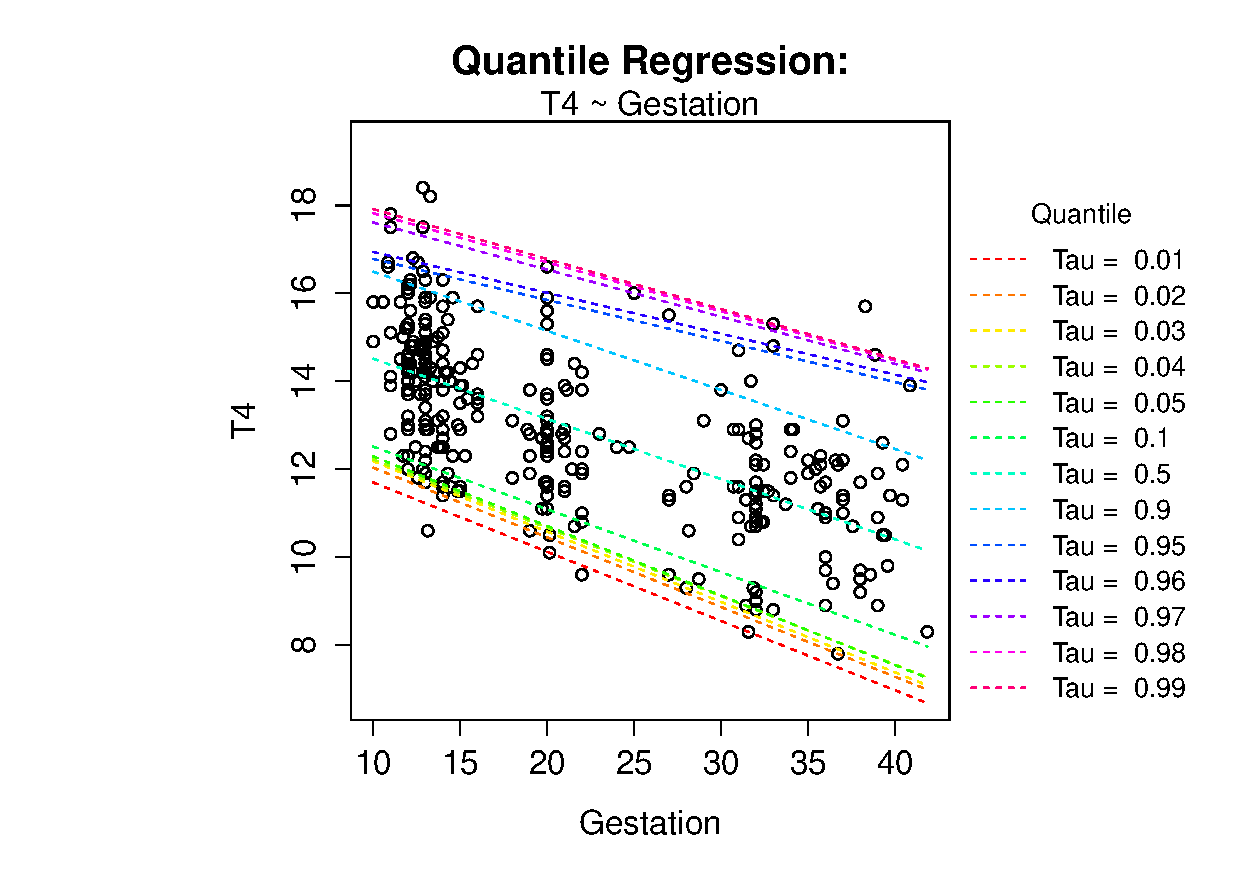
\includegraphics[width=9cm]{QRT4Model1.pdf}
    \caption{Simple Linear Model for free T4}
    \label{QR:T4Model1}
\end{figure}
\vspace{2mm}
\begin{figure}[ht]\centering
    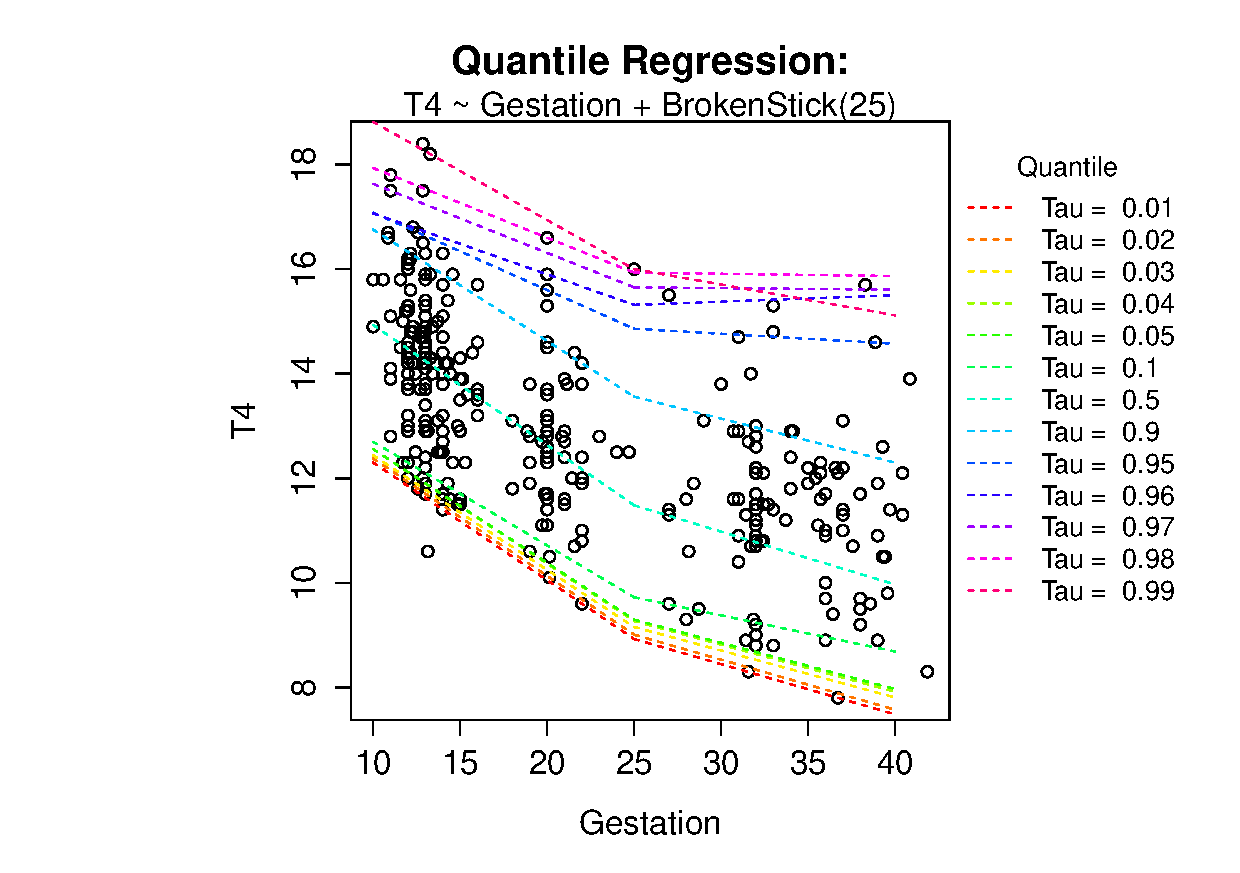
\includegraphics[width=9cm]{QRT4Model2.pdf}
    \caption{Broken Stick Model for free T4}
    \label{QR:T4Model2}
\end{figure}
\vspace{2mm}

However, from the scatterplot of free T$4$ v Gestation in figure \ref{QR:T4Model1}, it can be observed that free T$4$ has a prominent decline until approximately $25$ weeks gestation, after which free T$4$ levels begin to level off. To capture this additional piece of information, a ``Broken Stick" model was fitted with a change point at $25$ weeks gestation. The model is defined as follows
$$ T4 = \alpha + \beta_{1}(Gestation) + \beta_{2}(Gestation-25)^{+} + \epsilon $$
While this model appears to capture the change in trend of free T$4$ and improve the overall fit (figure \ref{QR:T4Model2}), it still has issues with overlapping quantile estimates. This issue will be addressed in the next chapter.

\subsection{Free T3}
Upon analysis of the free T$3$ variable earlier in this section it was shown that the data approximately followed a normal distribution and that no transformation of the data was required before modelling. Similar, to T$4$ a simple linear model of the form
$$ T3 = \alpha + \beta(Gestation) + \epsilon$$
was fitted to the data and the scatterplot in figure \ref{QR:T3Model1} was produced.
\vspace{2mm}

\begin{figure}[ht]\centering
    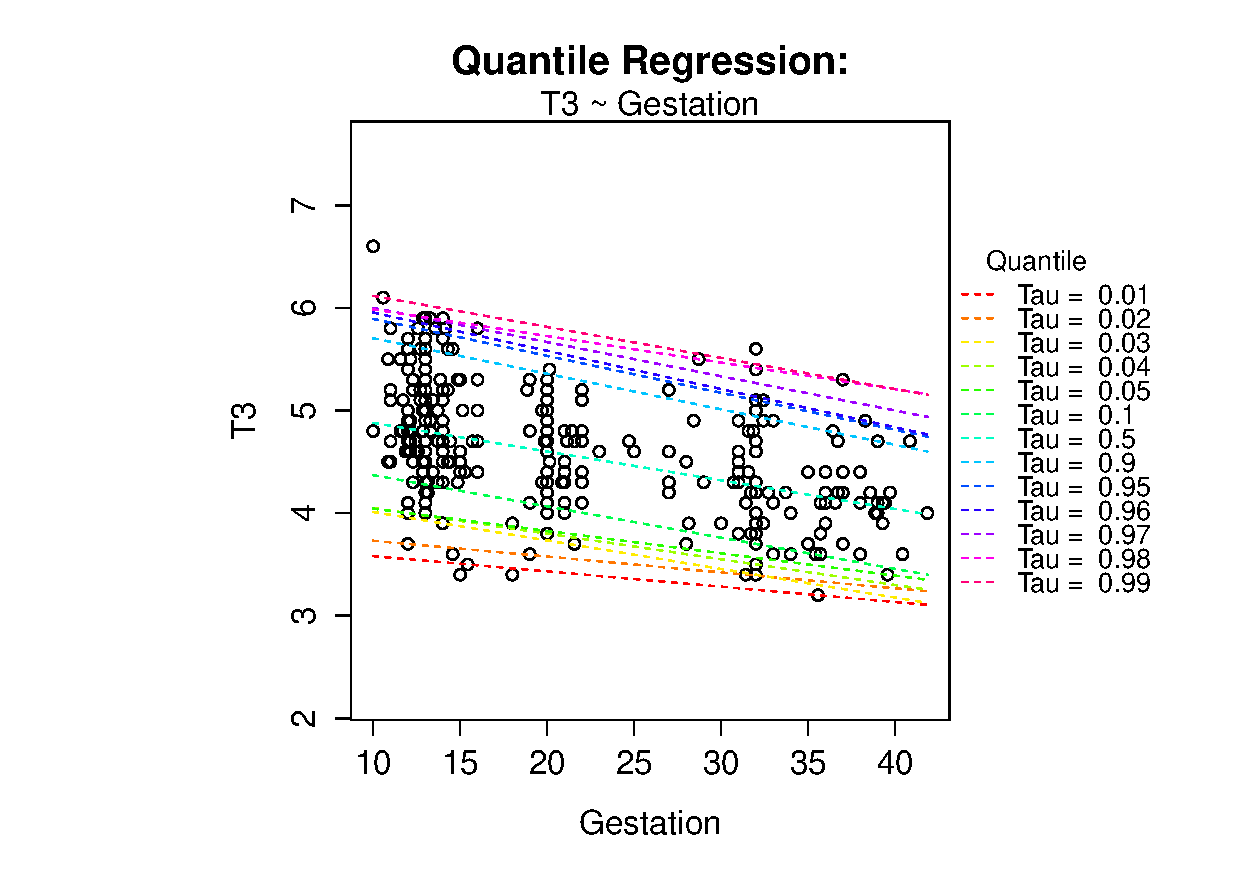
\includegraphics[width=9cm]{QRT3Model1.pdf}
    \caption{Linear Model for free T3}
    \label{QR:T3Model1}
\end{figure}
\vspace{2mm}

No clear patterns are clear from this scatterplot as was the case when viewing the initial model for T$4$, however a model of the form
$$ T3 = \alpha + \beta_{1}(Gestation) + \beta{2}(Gestation^{2}) + \epsilon$$
was fitted with the resultant plot shown in figure \ref{QR:T3Model2}.
\vspace{2mm}

\begin{figure}[ht]\centering
    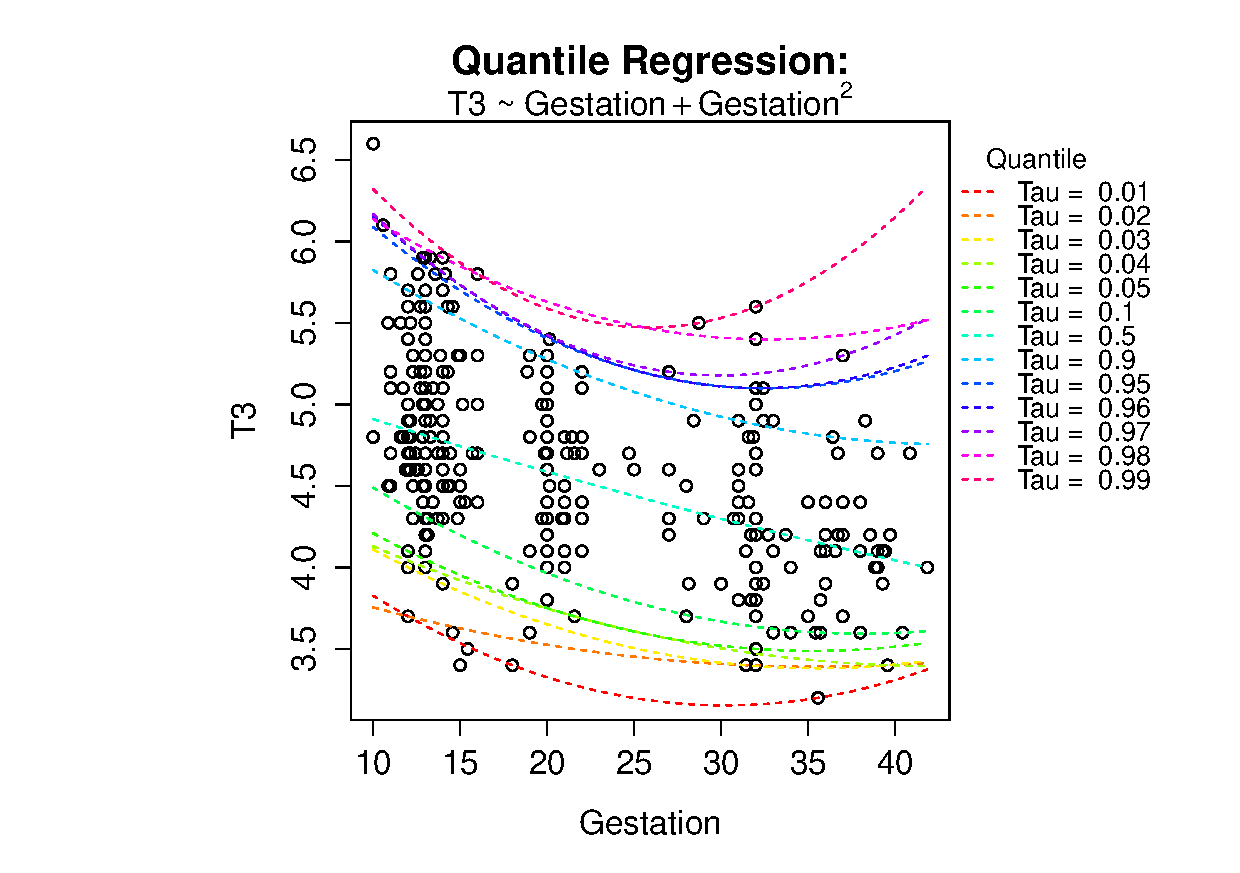
\includegraphics[width=9cm]{QRT3Model2.pdf}
   \caption{Quadratic Model for free T3}
    \label{QR:T3Model2}
\end{figure}
\vspace{2mm}

The quadratic model appears to have improved the fit of the data in comparison with the initial linear model that was fitted. However, even though this fit appears to model the data better the issue of quantile crossing is a dominant feature of the quadratic model plot.

\subsection{TSH}
Finally, a model will be fitted to establish the relationship between TSH and the week of gestation of patients. From the distribution analysis of TSH it was seen that the data was not normally distributed and so a square root transformation needed to be applied. The model took the form of
$$ \sqrt{TSH} = \alpha + \beta(Gestation) $$

\begin{figure}[ht]\centering
    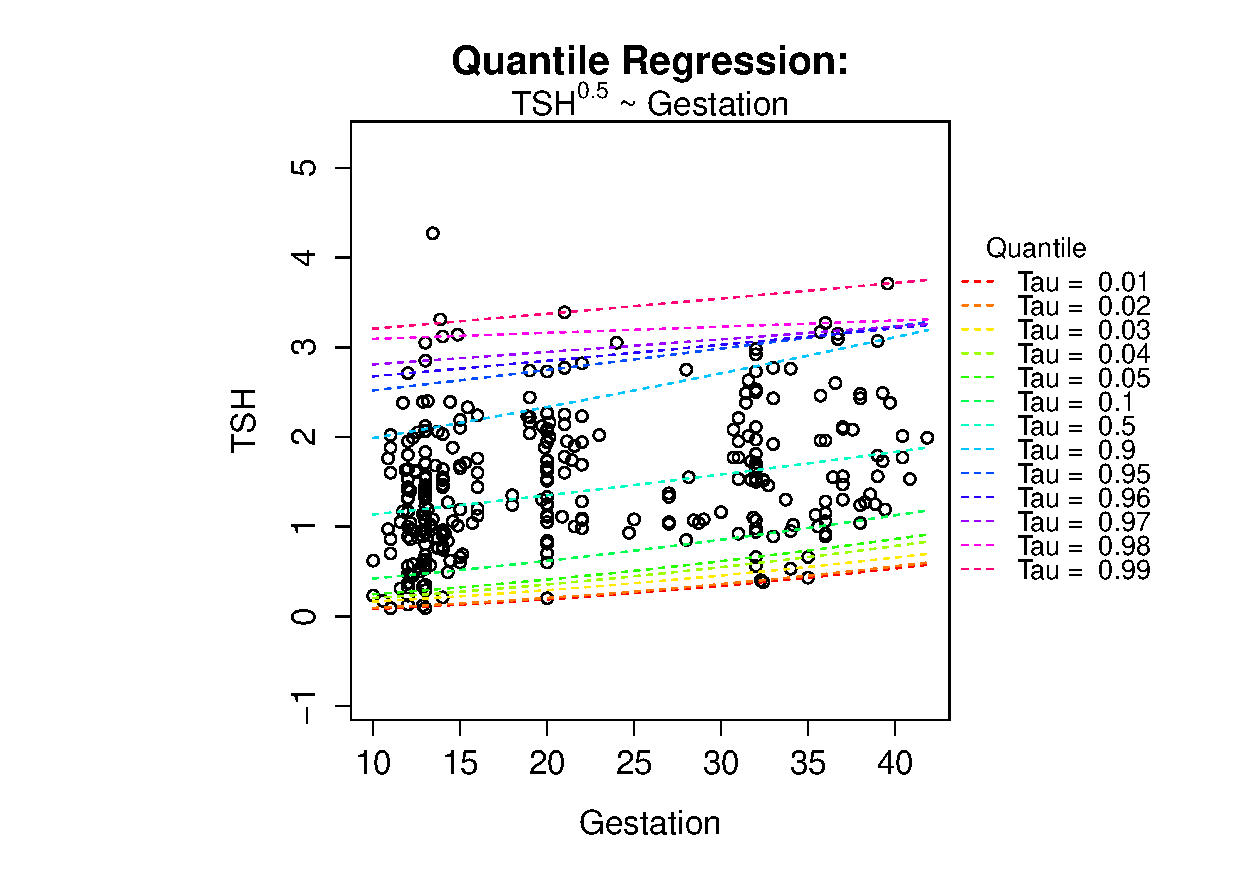
\includegraphics[width=9cm]{QRTSHModel1.pdf}
   \caption{Linear model for TSH}
    \label{QR:TSHModel1}
\end{figure}
\vspace{2mm}

The output from the model can be seen in figure \ref{QR:TSHModel1}. Again the regression quantile curves cross and while the model seems a good fit for the data this major issue makes it particularly hard to interpret sensible confident reference intervals for thyroid disease in pregnancy.

\chapter{Non-crossing Quantile Estimates}
As outlined previously, the major problem with quantile estimates for this data is the crossing of the quantile lines. Crossing quantile estimates make it impossible to assign an observation to a single reference range. For example, if we only treat the upper $5\%$ of the population and if the $0.95^{th}$ and the $0.90^{th}$ quantile estimates are crossing then how do we decide who to treat? If we assign a patient to be above the $0.95^{th}$ quantile estimate than they get treated but may not actually need the treatment. The opposite, which is much worse, could also occur, we assign a patient to be in the range between the $0.90^{th}$ and the $0.95^{th}$ quantile estimates, they do not receive the treatment and they do contract a thyroid disease. A simple example like this shows just how important non-crossing quantile estimates really are.

To address the problem, the intention is to use non-parametric approaches to calculating the quantile estimates. While some work has been carried out by others on the topic there exists no general off-the-shelf solution to the problem of overlapping quantile estimates. The solution provided uses a combination of linear programming constraints and b-spline functions.
\vspace{2mm}

\section{Theory behind Proposed Solution}
The objective function for quantile regression is defined as
$$ \hat{\beta}=\argmin_{\beta\in\Re^{p}}\sum\rho_{\tau}(y_{i}-x'\beta)$$
and thus the $\beta$ estimates are independent for each quantile estimated. That is to say that the $\beta$ estimates for $\tau=0.01$ are entirely independent of the $\beta$ estimates for $\tau=0.02$. This independent estimation of the quantiles allows for the possibility of crossing quantile curves, making classification of an individual to an interval impossible.
\vspace{2mm}

Crossing quantile occur when, for some values of $x$,
$$ \hat{y}_{\tau_{1}} = \hat{\beta}_{0}^{(\tau_{1})} + X \hat{\beta}^{(\tau_{1})} $$
intersects and crosses
$$ \hat{y}_{\tau_{2}} = \hat{\beta}_{0}^{(\tau_{2})} + X \hat{\beta}^{(\tau_{2})} $$
given that $0\leq\tau_{1}\leq\tau_{2}\leq1$. To eliminate the crossing of quantiles we require that
$$\hat{y}_{\tau_{1}} < \hat{y}_{\tau_{2}}$$
for all $x$ and all $\tau_{1}<\tau_{2}$. This in turn implies that
$$ \hat{\beta}_{0}^{(\tau_{1})} + X_{1} \hat{\beta}_{1}^{(\tau_{1})} + \ldots + X_{p} \hat{\beta}_{p}^{(\tau_{1})} < \hat{\beta}_{0}^{(\tau_{2})} + X_{1} \hat{\beta}_{1}^{(\tau_{2})} + \ldots + X_{p} \hat{\beta}_{p}^{(\tau_{2})} $$
which when simplified using matrix, notation results in
$$\tilde{X}[\beta_{\tau_{2}}-\beta_{\tau_{1}}]>0$$
where $\tilde{X}=[\mathbf{1} \; \mathbf{X}]$ and $\beta_{\tau_{i}}=[\beta_{0}^{\tau_{i}} \; \beta_{1}^{\tau_{i}} \; \ldots \; \beta_{p}^{\tau_{i}}]$.
\vspace{2mm}

One way to enforce that $\hat{\beta}_{\tau_{2}}-\hat{\beta}_{\tau_{1}}>0$ is to enforce that all $\hat{\beta}_{i}^{(\tau_{2})}>\hat{\beta}_{i}^{(\tau_{1})}$, during the linear programming stage in which the quantiles are calculated. The Frisch-Newton adaption of the simplex method allows such a constraint to be added to the optimisation problem. The Frisch-Newton allows a $\;\geq\;$ constraint to be set, as a result the constraint used here will be $\hat{\beta}_{i}^{(\tau_{2})}\geq\hat{\beta}_{i}^{(\tau_{1})}+\epsilon$, where epsilon is of the order of $3.6\:\times\:10^{-11}$. $\epsilon$ is included to act as a correction factor after including a $\;\geq\;$ constraint instead of a $\;>\;$ constraint.  In concise notation, the proposed solution is to solve the following optimisation problem
$$\hat{\beta}=\argmin_{\beta\in\Re^{p}}\sum\rho_{\tau}(y_{i}-x'\beta)$$
subject to the constraint $\hat{\beta}_{(\tau_{i})}\geq\hat{\beta}_{(\tau_{i-1})}+\epsilon$ for $0<\tau<1$.
\vspace{2mm}

The approach thus far attempts to estimate the current quantile by constraining the coefficients to be greater than the coefficients of the previous estimated quantile. While carrying out quantile regression analysis in this fashion will remove crossing in quantiles it will not produce optimal solutions. The asymptotic variance of a quantile estimator is proportional to
$$\frac{\tau(1-\tau)}{f(F^{-1}(\tau))}$$
where $f(\cdot)$ is the pdf of the error distribution and $F(\cdot)$ is the cdf of the error distribution.
\vspace{2mm}

For the normal distribution, it can be shown that the asymptotic variance is minimised at $\tau\:=\:0.5$. Thus the estimated quantile at $\tau\:=\:0.5$ is relatively more accurate than other estimated quantiles. From this result it makes sense to estimate the quantiles by starting at the median regression line and working out to the smaller quantiles, in both directions. The solution proposed here incorporates this feature and estimates the $0.5^{th}$ quantile even if it is not required as a quantile of interest. For quantiles greater than the median the original constraint remains valid, while no constraint is no applied to the median quantile. However, the constraint needs to be changed for quantiles less than the median quantile. The constraint required is
$$\hat{\beta}_{(\tau_{i})}\leq\hat{\beta}_{(\tau_{i+1})}-\epsilon$$
however, the Frisch-Newton method does not allow $\:\leq\:$ constraints to be set and so the constraint which is used is
$$-\hat{\beta}_{(\tau_{i})}\geq-\hat{\beta}_{(\tau_{i+1})}+\epsilon$$
\vspace{1mm}

In short the solution proposed here applies constraints to the original optimisation problem to eradicate the issue of quantiles crossing, thus allowing simpler classification of individuals to a range. The proposed solution results in the optimisation problem with constraints taking the form of,


$$\hat{\beta}=\argmin_{\beta\in\Re^{p}}\sum\rho_{\tau}(y_{i}-x'\beta)$$
\[\text{subject to} \;
    \begin{cases}
        -\hat{\beta}_{(\tau_{i})}\geq-\hat{\beta}_{(\tau_{i+1})}+\epsilon,& \text{if } 0<\tau<0.5, \\
        \text{no constraints},& \text{if } \tau=0.5,\\
        \hat{\beta}_{(\tau_{i})}\geq\hat{\beta}_{(\tau_{i-1})}+\epsilon,& \text{if } 0.5<\tau<1
    \end{cases}
\]
\vspace{2mm}

\section{Implementation of Proposed Solution in R}
The solution proposed here has been implemented in {\small{\verb"R"}}, the code for which is provided in Appendix \ref{App:QRFunction}. Roger Koenker's {\small{\verb"quantreg"}} package provided a basis for the implementation of the method and the Frisch-Newton simplex code is adapted from this package. \vspace{2mm}

The code provided as a solution to the issue of crossing quantiles is broken into $7$ key sections which are outlined in the following list. The following also details the tasks carried out in each step and how they contribute to the overall solution of the problem.

\begin{enumerate}[1)]
    \item \textbf{Read Model Arguments}
    \\ The code {\small{\verb"QR(formula, tau, data)"}} calls the function for non-crossing quantiles. The {\small{\verb"formula"}} argument takes the form {\small{\verb"Y ~ X"}}, just as it did in the examples provided in Chapter \ref{Background}. The {\small{\verb"tau"}} argument accepts single tau values to be estimated or a vector of tau to be estimated. The {\small{\verb"data"}} argument takes the name of the dataset from which the variables of interest come from. \\
    The model arguments are read into a {\small{\verb"model.frame"}} object, this object will contain the dependent and independent variables and will act as the data frame for the entire analysis. In this section, checks are also carried out to ensure that the design matrix is not singular, if the design matrix is singular computation is stopped and a warning returned to the user.
    \item \textbf{Load required packages, constants and functions}
    \\ This section of the code installs and loads the required {\small{\verb"quantreg"}} package, so that the {\small{\verb"rq.fit"}} fortran code is available for the calculations of the quantiles. The check function denoted by $\rho_{\tau}(u)$ is also defined here, more information on the check function can be found in Chapter \ref{Background:FA}. Finally, $\epsilon$ is also defined in this section to be a value of {\small{\verb".Machine$double.eps^(2/3)"}} which is equivalent to $3.666853\; \times \;10^{-11}$.
    \item \textbf{Check validity of inputted taus}
    \\ As discussed earlier the tau values required for quantile regression must be in the range $0<\tau<1$, this section of code ensures this constraint is satisfied and stops computation if it is not. As users specifing $\tau=0$ or $\tau=1$ is likely, these requests do not throw an error but rather $\tau=0$ becomes $\tau=\epsilon$ and $\tau=1$ becomes $\tau=1-\epsilon$.
    \item \textbf{Define required data objects}
    \\ All data objects to hold the relevant output is defined here based on the number of tau values which we are interested in. A matrix, {\small{\verb"coef"}}, of size $n\:\times\:p$ is defined for the coefficients, where $n$ is the number of tau values of interest and $p$ is the number of model parameters plus one to include the intercept. A vector, {\small{\verb"rho"}}, is defined to hold the value of the check function for each of the specified quantiles. Finally, two matrices, {\small{\verb"fitted"}} and {\small{\verb"resid"}}, are defined to hold the fitted values and the residuals respectively, each of size $n\:\times\:d$, where $d$ is the number of observations in the data.
    \item \textbf{Calculate regression quantiles}
    \\ The calculation of the regression quantiles is carried out in full in this section. There is two different approaches depending on the number of quantiles required.
    \\If only one tau is specified in the model arguments then the function will return the relevant output for that single quantile model. In this case no constraints are applied to the coefficients as non-crossing is gaurenteed when only one quantile is of interest.
    \\If more than one tau is of interest in the analysis then the first step is to calculate the median regression quantile, weather it is of interest or not. The tau values are then split into two subsets, one set will contain the taus with values greater than 0.5 while the other will contain the taus with values less than 0.5. The quantiles will then be estimated with the correct constraints applied. A call to the {\small{\verb"rq.fit.fnc"}} function in the {\small{\verb"quantreg"}} package with the correct constraints results in the calculation of each $\tau^{th}$ quantile required by the user.
    \item \textbf{Tidy up the output}
    \\ The output is formatted into tables to make output from the function concise and clear.
    \item \textbf{Return the required information}
    \\ The required output is returned as a single variable which has multiple components, including the coefficients, fitted values, residuals, check function values and more, for each tau specified. Each individaul component can be accessed using the \$ symbol in {\small{\verb"R"}}, for example if {\small{\verb"model"}} is an object produced by {\small{\verb"QR"}} then {\small{\verb"model$coef"}} will return the coefficients for that object.
\end{enumerate}
\vspace{2mm}

\par\noindent
The entire code for the function, which is commented, is provided in Appendix \ref{App:QRFunction}.
\section{Application to thyroid data}
In this section, the thyroid data, which this project is based upon, will be revisited and in particular the models specified for T3, T4 and TSH will be reviewed. The models will then be fitted using the proposed solution to non-crossing quantiles provided in this chapter, to provide a real-life example of this method in action.
\vspace{2mm}

The T3 hormone variable appeared to be curve linear from the analysis in Chapter \ref{ThyroidReg} and so a model of the form
$$T3=\beta_{0}+\beta_{1}(Gestation)+\beta_{2}(Gestation^{2})+\epsilon$$
was fitted. However, crossing quantiles were still evident in figure \ref{QR:T3Model2} and so reference ranges were still impossible to specify exactly. Using the same model and calculating the same quantile curves, using the new method outlined above results in figure \ref{NCQR:T3}.
\vspace{2mm}
\begin{figure}[ht]\centering
    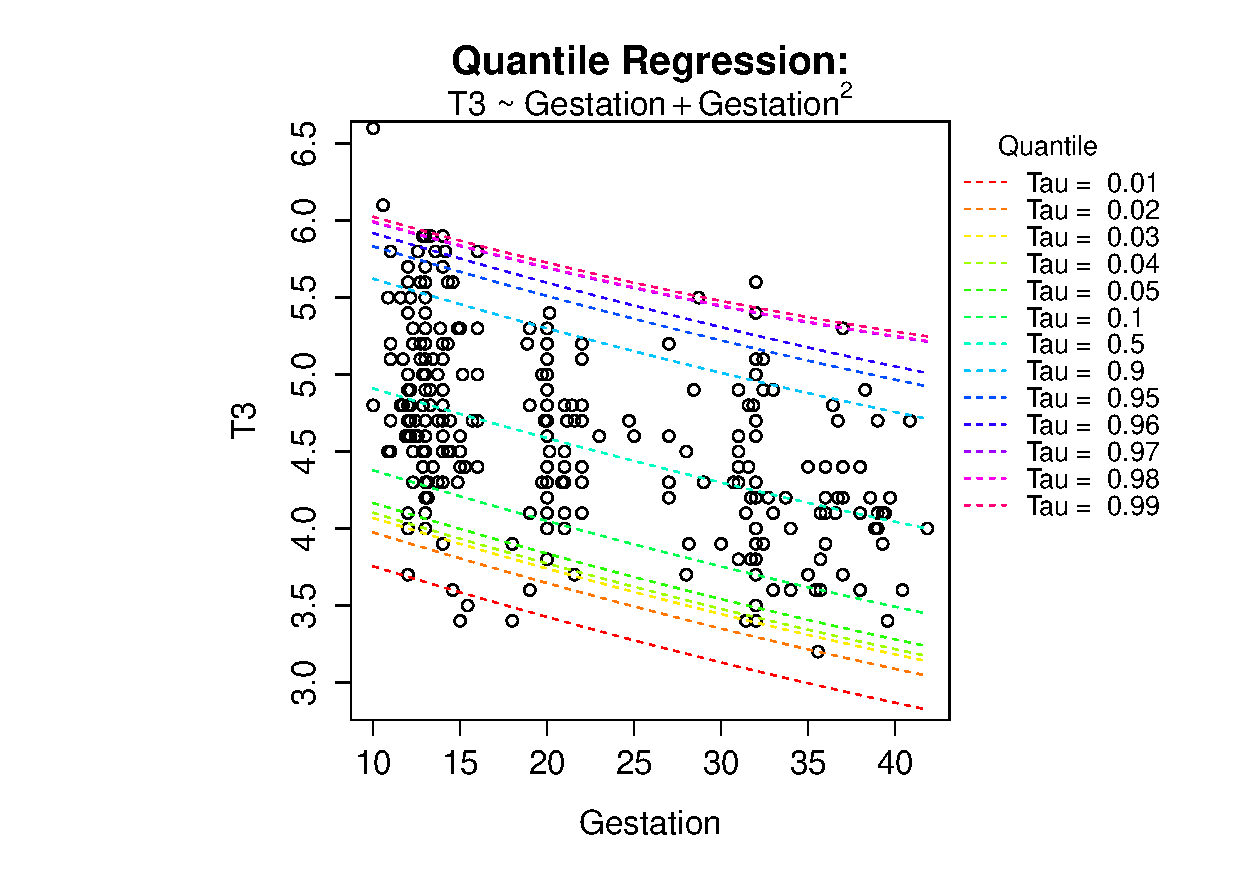
\includegraphics[width=10cm]{QRT3NCModel.pdf}
    \caption{Non-crossing quantile curves for T3}
    \label{NCQR:T3}
\end{figure}
\vspace{2mm}
The quantiles never cross in this graphic and as a result it is possible to differentiate between individuals which belong to different reference ranges. This allows doctors to treat those who need to be treated and also to not treat those who do not require treatment.
\vspace{2mm}

\begin{figure}[ht]\centering
    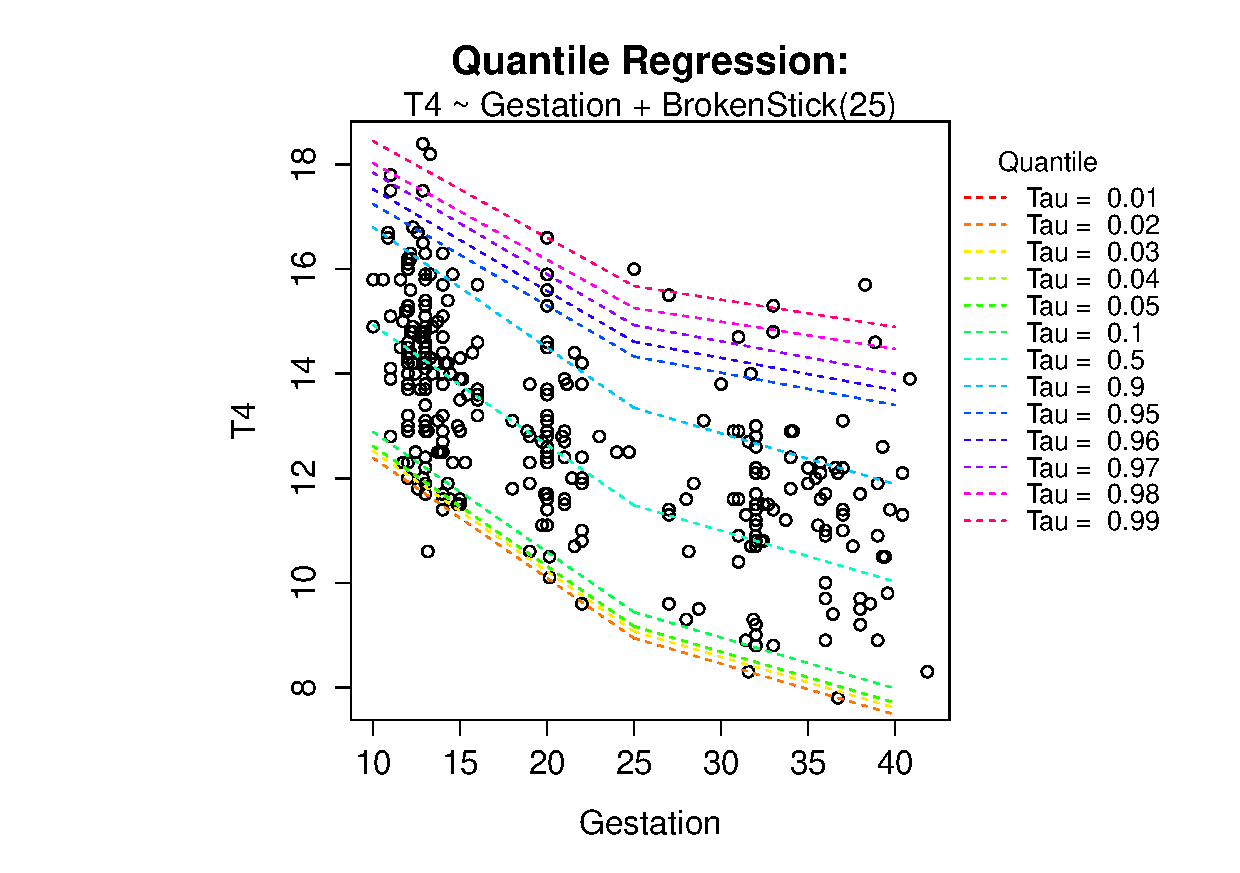
\includegraphics[width=10cm]{QRT4NCModel.pdf}
    \caption{Non-crossing quantile curves for T4}
    \label{NCQR:T4}
\end{figure}
\vspace{2mm}

It was found that the T4 hormone variable was best modelled using a "Broken Stick" model as due to a significant change in slope of the data at 25 weeks gestation. The model fitted was
$$T4=\beta_{0}+\beta_{1}(Gestation)+\beta_{2}(Gestation-25)^{+}+\epsilon$$
where $(\cdot)^{+}$ is the $\max(0,\cdot)$.
Calculating the quantile curves for this model using the non-crossing quantile approach results in figure \ref{NCQR:T4}. As expected, the quantile curves never cross in this graphic and as before the reference ranges are now easier to specify. In the case of thyroid disease it is easier to identify those patients who lie in the upper and lower $2\%$ ranges, who require treatment.
\vspace{2mm}

Finally, the TSH hormone variable required a box-cox transformation before modelling and the best fitting model was
$$ \sqrt{TSH} = \alpha + \beta(Gestation)$$
As was the issue with all the model fittings in Chapter \ref{ThyroidReg} crossing quantiles did not allow classification of some individuals to a single reference range. Applying the algorithm described in this chapter to the TSH hormone variable using the model specified resulted in figure \ref{NCQR:TSH}, with no crossing quantiles evident, the algorithm has again performed to requirements.
\vspace{2mm}
\begin{figure}[ht]\centering
    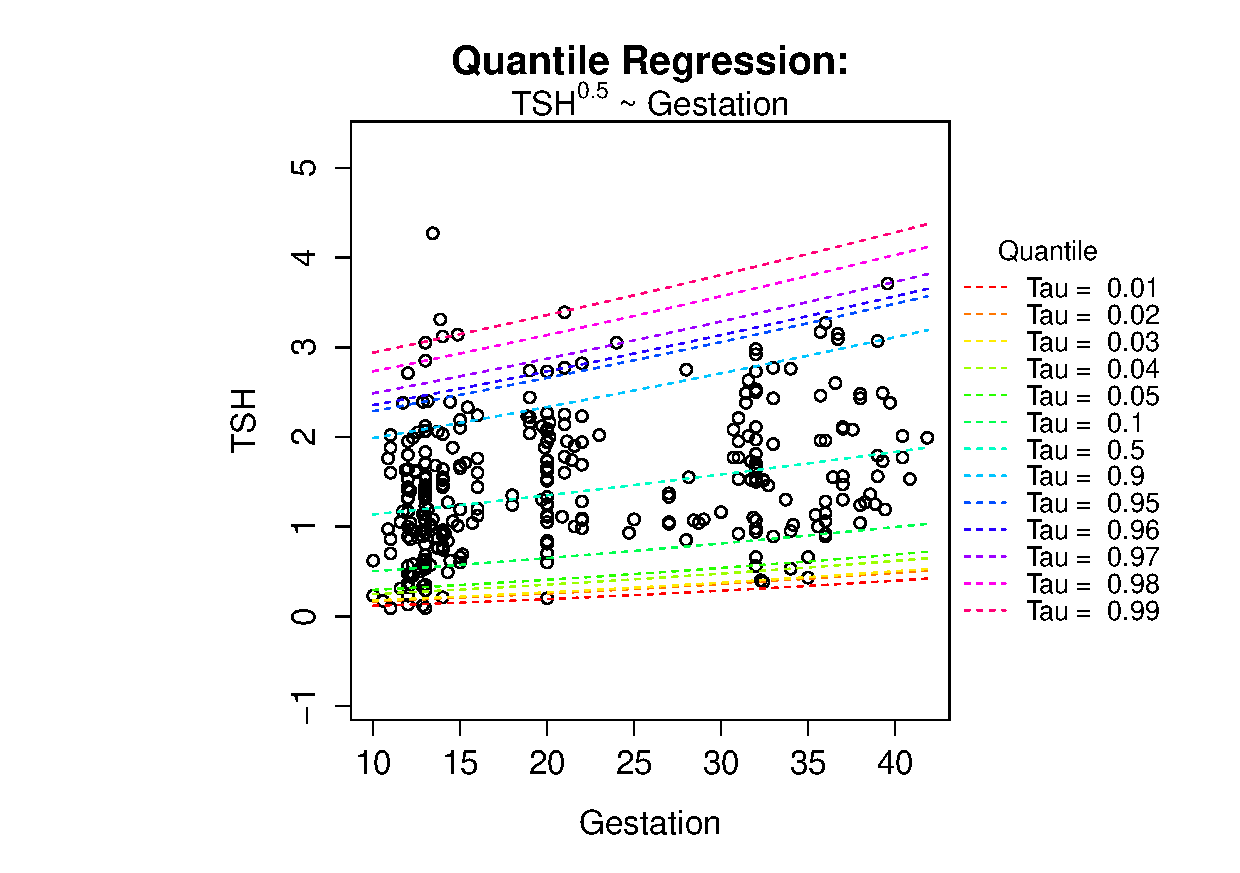
\includegraphics[width=10cm]{QRTSHNCModel.pdf}
    \caption{Non-crossing quantile curves for TSH}
    \label{NCQR:TSH}
\end{figure}
\vspace{2mm}

\par\noindent
The code used to produce all of the above graphics can be found in Appendix \ref{App:QRFunctionThyroid}.

 % This isn't actually required just here to tidy all commands into their own nest
\newpage
\addcontentsline{toc}{chapter}{References}
\bibliography{Report}
\bibliographystyle{chicago}

\newpage
\appendix
\addcontentsline{toc}{chapter}{Appendix}

\chapter{R code for Engel Data Example}

\section{Quantreg Code}\label{App:Engel-Code-Quantreg}
\begin{lstlisting}
# Quantreg Package: Simulation on Sample Data

 # log transformation of Data: TRUE/FALSE

  logTrans <- FALSE

 # Loading data and packages

 library(quantreg)
 library(ggplot2)
 data(engel)
 attach(engel)

 if(logTrans==TRUE){
    x <- log10(engel$income)
    y <- log10(engel$foodexp)
 }else{
    x <- engel$income
    y <- engel$foodexp
 }

 # Creating a data frame of quantile regression lines

 mdl.quant <- rq(y ~ x,tau=c(0.05,0.1,0.25,0.5,0.75,0.9,0.95))
 quant.results <- data.frame(t(coef(mdl.quant)))
 colnames(quant.results) <- c("Intercept", "Slope")

 # Creating a linear model to compare to quantiles (median)

 linear.quant <- lm(y ~ x)

 # Creating a data set to output to a latex table

 quant.results[8,1] <- linear.quant$coefficients[1]
 quant.results[8,2] <- linear.quant$coefficients[2]

 quant.results[,"Names"] <- c("Tau = 0.05", "Tau = 0.10",
                          "Tau = 0.25", "Median", "Tau = 0.75",
                            "Tau = 0.90", "Tau = 0.95", "Mean")

 quant.results <- data.frame(quant.results[,"Names"],
                          round(quant.results[,"Intercept"],3),
                              round(quant.results[,"Slope"],3))
 colnames(quant.results) <- c("Quantile", "Intercept", "Slope")

 # Plotting points and the quantile regression lines

 if(logTrans==TRUE){
    title <-"quantreg package: rq function (log transform)"
 }else{
    title <-"quantreg package: rq function"
 }

 plt.quant <- qplot(x=x, y=y, xlab="Household Income",
                    ylab="Food Expenditure", main=title) +
            geom_abline(aes(intercept=Intercept, slope=Slope,
            color=Quantile),show_guide=TRUE,data=quant.results)
\end{lstlisting}

\section{BayesQR Code}\label{App:Engel-Code-bayesQR}
\begin{lstlisting}
# BayesQR Package: Simulation on Sample Data

  # log transformation of Data: TRUE/FALSE

  logTrans <- FALSE

  # Loading data and packages

  library(bayesQR)
  library(ggplot2)
  library(quantreg)
  data(engel)
  attach(engel)

  if(logTrans==TRUE){
    x <- log10(engel$income)
    y <- log10(engel$foodexp)
  }else{
    x <- engel$income
    y <- engel$foodexp
  }
  # Creating a data frame of quantile regression lines

  taus <- c(0.05,0.1,0.25,0.5,0.75,0.9,0.95)
  intercept <- c(rep(0,7))
  slope <- c(rep(0,7))

  mdl.bays <- bayesQR(y ~ x, quantile=taus, ndraw=5000)

  sum <- summary(mdl.bays, burnin=500)

  for(i in 1:length(sum)){
    intercept[i] <- sum[[i]]$betadraw[1,1]
    slope[i] <- sum[[i]]$betadraw[2,1]
  }

  bays.results <- data.frame(cbind(intercept,slope))
  colnames(bays.results) <- c("Intercept", "Slope")

  # Creating a linear model to compare to quantiles (median)

  linear.bays <- lm(y ~ x)
  bays.results[8,1] <- linear.bays$coefficients[1]
  bays.results[8,2] <- linear.bays$coefficients[2]

  bays.results[,"Names"] <- c("Tau = 0.05","Tau = 0.10",
                        "Tau = 0.25","Median","Tau = 0.75",
                            "Tau = 0.90","Tau = 0.95","Mean")

  bays.results <- data.frame(bays.results[,"Names"],
                        round(bays.results[,"Intercept"],4),
                            round(bays.results[,"Slope"],4))
  colnames(bays.results) <- c("Quantile", "Intercept", "Slope")

  # Plotting points and the quantile regression lines

  if(logTrans==TRUE){
    title <-"bayesQR package: bayesQR function (log transform)"
  }else{
    title <-"bayesQR package: bayesQR function"
  }

  plt.bays <- qplot(x=x, y=y, xlab="Household Income",
                     ylab="Food Expenditure",main=title) +
    geom_abline(aes(intercept=Intercept, slope=Slope,
            color=Quantile),show_guide=TRUE, data=bays.results)

\end{lstlisting}

\section{Lqmm Code}\label{App:Engel-Code-lqmm}
\begin{lstlisting}
# lqmm Package: Simulation on Sample Data

 # log transformation of Data: TRUE/FALSE

 logTrans <- FALSE

 # Loading data and packages

 library(lqmm)
 library(ggplot2)
 library(quantreg)
 data(engel)
 attach(engel)

 if(logTrans==TRUE){
    x <- log10(engel$income)
    y <- log10(engel$foodexp)
 }else{
    x <- engel$income
    y <- engel$foodexp
 }
 # Creating a data frame of quantile regression lines

 mdl.mix <- lqm(y ~ x,iota=c(0.05,0.1,0.25,0.5,0.75,0.9,0.95))
 mix.results <- data.frame(t(coef(mdl.mix)),row.names=NULL)
 colnames(mix.results) <- c("Intercept", "Slope")

 # Creating a linear model to compare to quantiles (median)

 linear.mix <- lm(y ~ x)
 mix.results[8,1] <- linear.mix$coefficients[1]
 mix.results[8,2] <- linear.mix$coefficients[2]

 mix.results[,"Names"] <- c("Tau = 0.05", "Tau = 0.10",
                         "Tau = 0.25", "Median", "Tau = 0.75",
                          "Tau = 0.90", "Tau = 0.95", "Mean")

 mix.results <- data.frame(mix.results[,"Names"],
                        round(mix.results[,"Intercept"],4),
                         round(mix.results[,"Slope"],4))
 colnames(mix.results) <- c("Quantile", "Intercept", "Slope")

 # Plotting points and the quantile regression lines

 if(logTrans==TRUE){
    title <- "lqmm package: lqm function (log transform)"
 }else{
    title <- "lqmm package: lqm function"
 }

 plt.mix <- qplot(x=x, y=y, xlab="Household Income",
                ylab="Food Expenditure", main=title) +
            geom_abline(aes(intercept=Intercept, slope=Slope,
            color=Quantile), show_guide=TRUE, data=mix.results)

\end{lstlisting}

\chapter{R Code for Chapter 3}
\section{Distributions}\label{App:Distributions}
\begin{lstlisting}
 ##### Distribution Analysis: Graph + Normality Test #####
 #                                                       #
 # Author: Kevin Brosnan                                 #
 # Date: 24/02/2014                                      #
 #                                                       #
 # Description:                                          #
 #  1) Histogram                                         #
 #  2) Boxplot                                           #
 #  3) QQ-plots                                          #
 #  4) Shapiro-Wilk Test                                 #
 #                                                       #
 # # # # # # # # # # # # # # # # # # # # # # # # # # # # #

 distribution <- function(data){

   name <- deparse(substitute(data))
   split.screen(figs=c(2,1))
   split.screen(figs=c(1,2), screen=1)

   screen(3)
     # Box-Plot of Data
     titleBox <- paste("Boxplot of ", name)
     boxplot(data, main=titleBox)
   screen(4)
     # QQ-plot of data
     qqnorm(data)
     qqline(data, col="red")
   screen(2)
     # Histogram of Data
     titleHist <- paste("Histogram of ", name)
     hist(data, xlab=name, main=titleHist)

   close.screen(all.screens=TRUE)

   normtest <- shapiro.test(data)
   return(normtest)
 }

 distribution(T4)
 distribution(T3)
 distribution(TSH)
\end{lstlisting}

\section{Box-Cox} \label{App:BoxCox}
\begin{lstlisting}
 #####   Box-Cox Power Transformation Calculation    #####
 #                                                       #
 # Author: Kevin Brosnan                                 #
 # Date: 19/02/2014                                      #
 #                                                       #
 # Description:                                          #
 #  1) Produce a plot of lambda v's log-likelihood       #
 #  2) Return the exact value of lambda to the user      #
 #  3) Return suggested values of lambda to user         #
 #                                                       #
 # # # # # # # # # # # # # # # # # # # # # # # # # # # # #

 box.cox <- function(formula, plotit=TRUE){

   # Checking the class of the formula argument passed
   # to the function

     if(class(formula)=="lm"){
       formula <- update(object, y=TRUE, qr=TRUE)
     }else if(class(formula)=="formula"){
       formula <- lm(formula, y=TRUE, qr=TRUE)
     }else{
       stop("Formula must be of class formula or of class lm")
     }

     y <- formula$y
     xqr <- formula$qr

   # Make sure response variable y is positive

     if(any(y<=0)){
       stop("Response variable must be positive")
     }

   # Box-Cox Algorithm

     lambda <- seq(-2,2,length=length(y))
     eps <- 0.02

     n <- length(y)
     y <- y/exp(mean(log(y)))
     logy <- log(y)

     xl <- loglik <- as.vector(lambda)
     m <- length(xl)

     for(i in 1:m){
       if(abs(la <- xl[i]) > eps){
         yt <- (y^la - 1)/la
       }else{
         yt <- logy*(1 + (la*logy)/2*(1 + (la*logy)/3*
                                    (1 + (la*logy)/4)))
       }
       loglik[i] <- -n/2 * log(sum(qr.resid(xqr, yt)^2))
     }

   # Calculating maximum values of lambda and log-likelihood

     max_index <- which(loglik==max(loglik))
     Loglik_max <- loglik[max_index]
     lambda_max <- xl[max_index]

   # Plotting log-likelihood vs Lambda

     if(plotit){

       lim <- Loglik_max - qchisq(19/20, 1)/2

       ind <- range((1:m)[loglik>lim])
       xlim <- c(0,0)

       if(loglik[1] < lim){
         i <- ind[1]
         xlim[1] <- xl[i-1] + ((lim - loglik[i-1])*
            (xl[i] - xl[i-1]))/(loglik[i] - loglik[i-1])
       }

       if(loglik[m] < lim){
         i <- ind[2]
         xlim[2] <- xl[i-1] + ((lim - loglik[i-1])*
            (xl[i] - xl[i-1]))/(loglik[i] - loglik[i-1])
       }

       xlim <- sort(xlim)

       xlower <- which(xl >= xlim[1]-0.01)
       xupper <- which(xl >= xlim[2]+0.01)

       xlower <- xlower[1]
       xupper <- xupper[1]

       dev.hold()
       on.exit(dev.flush())

       plot(x=xl[xlower:xupper], y=loglik[xlower:xupper],
                xlab=expression(lambda),ylab="log-Likelihood",
                 type="l",  xlim=c(xlim[1]-0.01,xlim[2]+0.01))

       title(main="Box-Cox Transformation")

       plims <- par("usr")
       scal <- (1/4 * (plims[4]-plims[3]))/par("pin")[2]

       abline(h=lim, lty=3)
       text <- bquote(lambda*"="*.(round(lambda_max,2)))
       text(lambda_max, Loglik_max - scal, text, col="red")

       y0 <- plims[3]

       if(max_index>1 && max_index<m){
         segments(lambda_max, y0, lambda_max, Loglik_max,lty=3)
       }

       segments(xlim[1], y0, xlim[1], lim, lty=3)
       segments(xlim[2], y0, xlim[2], lim, lty=3)
     }

   # Outputting best suggestion for lambda

     lambda_suggestion <- FALSE

     if(abs(lambda_max)>0.4 && abs(lambda_max)<0.6){
       lambda_suggestion <- TRUE
       if(lambda_max<0){
         lambda_sug <- "1/sqrt(y)"
       }else{
         lambda_sug <- "sqrt(y)"
       }
     }else if(abs(lambda_max)>0.9 && abs(lambda_max)<1.1){
       lambda_suggestion <- TRUE
       if(lambda_max<0){
         lambda_sug <- "1/y"
       }else{
         lambda_sug <- "y"
       }
     }else if(abs(lambda_max)<0.1){
       lambda_suggestion <- TRUE
       lambda_sug <- "ln(y)"
     }

     if(lambda_suggestion){
       out <- sprintf("The optimal value of lambda to use in
            transforming the supplied data is lambda = %.2f.
            However a %s transformation would be easier to
            interpret and apply", lambda_max, lambda_sug)
     } else{
       out <- sprintf("The optimal value of lambda to use in
            transforming the supplied data is lambda = %.2f",
                                         lambda_max)
     }

   # Returning final values
     print(out)
     invisible(list(x=xl, y=loglik, lambda=lambda_max))
 }

 box.cox(TSH, plotit=TRUE)
\end{lstlisting}
\section{Linear Quantile Models} \label{App:QuantileModels}
\subsection*{free T4}\label{App:QuantileModelsT4}
\begin{lstlisting}
#####               T4 Model Fitting                #####
#                                                       #
# Author: Kevin Brosnan                                 #
# Date: 21/02/2014                                      #
#                                                       #
# Description:                                          #
#  Modelling T4 v Gestation initially with a linear     #
#  model and then including a "Broken Stick" element    #
#                                                       #
# # # # # # # # # # # # # # # # # # # # # # # # # # # # #

  taus <- c(0.01,0.02,0.03,0.04,0.05,0.1,
                0.5,0.9,0.95,0.96,0.97,0.98,0.99)

  # T4 Model 1

  modT4_1 <- rq(T4 ~ Gestation, data=thyroid, tau=taus)
  plot.QR(modT4_1,x=Gestation, y=T4)

  # T4 Model 2
  temp <- Gestation
  for(i in 1:length(Gestation)){
    if(Gestation[i]>=25){
      temp[i] <- Gestation[i] - 25
    }else{
      temp[i] <- 0
    }
  }

  modT4_2 <- rq(T4 ~ Gestation + temp,
                        data=thyroid, tau=taus)
  plot(y=T4, x=Gestation)

  col <- rainbow(length(taus))
  for(i in 1:length(taus)){
    curve(from=10,to=25,modT4_2$coef[1,i]+x*modT4_2$coef[2,i],
                            add=TRUE,lty=2, col=col[i])
    curve(from=25, to=40,modT4_2$coef[1,i]+x*modT4_2$coef[2,i]
            +(x-25)*modT4_2$coef[3], lty=2,col=col[i],add=TRUE)
  }
  title(main="Quantile Regression:", cex=1.5)
  mtext("T4 ~ Gestation + BrokenStick(25)",cex=1)
  labels <- rep("", length(modT4_2$tau))

  for(i in 1:length(modT4_2$tau)){
    labels[i] <- paste("Tau = ", modT4_2$tau[i])
  }

  par(xpd=TRUE)
  legend((max(Gestation)+1),max(T4, na.rm=TRUE),
    labels, cex=0.8, col=col, lty=2, title="Quantile",bty="n")
\end{lstlisting}
\subsection*{free T3}\label{App:QuantileModelsT3}
\begin{lstlisting}
#####               T3 Model Fitting                #####
#                                                       #
# Author: Kevin Brosnan                                 #
# Date: 21/02/2014                                      #
#                                                       #
# Description:                                          #
#  Modelling T3 v Gestation initially with a linear      #
#  model and then a quadratic model                     #
#                                                       #
# # # # # # # # # # # # # # # # # # # # # # # # # # # # #

taus <- c(0.01,0.02,0.03,0.04,0.05,0.1,
                        0.5,0.9,0.95,0.96,0.97,0.98,0.99)

  # T3 Model 1

  modT3_1 <- rq(T3 ~ Gestation, data=thyroid, tau=taus)
  plot.QR(modT3_1,x=Gestation, y=T3)

  # T3 Model 2

  modT3_2 <- rq(T3 ~ Gestation + I(Gestation^2),
                        data=thyroid, tau=taus)
  plot(x=Gestation, y=T3)

  col <- rainbow(length(taus))
  for(i in 1:length(taus)){
    curve(modT3_2$coef[1,i]+x*modT3_2$coef[2,i]+(x^2)
            *modT3_2$coef[3,i],add=TRUE,lty=2, col=col[i])
  }

  title(main="Quantile Regression:", cex=1.5)
  subtitle <- bquote(T3*" ~ "*Gestation + Gestation^2)
  mtext(subtitle,cex=1)

  labels <- rep("", length(modT4_2$tau))

  for(i in 1:length(modT4_2$tau)){
    labels[i] <- paste("Tau = ", modT4_2$tau[i])
  }

  par(xpd=TRUE)
  legend((max(Gestation)+1),max(T3, na.rm=TRUE),labels,
             cex=0.8, col=col, lty=2, title="Quantile",bty="n")
\end{lstlisting}
\subsection*{TSH}\label{App:QuantileModelsTSH}
\begin{lstlisting}
#####             TSH Model Fitting                 #####
#                                                       #
# Author: Kevin Brosnan                                 #
# Date: 21/02/2014                                      #
#                                                       #
# Description:                                          #
#  Modelling TSH v Gestation                            #
#                                                       #
# # # # # # # # # # # # # # # # # # # # # # # # # # # # #

  taus <- c(0.01,0.02,0.03,0.04,0.05,0.1,
                0.5,0.9,0.95,0.96,0.97,0.98,0.99)

  # TSH Model

  modTSH <- rq(TSH^0.5 ~ Gestation,
                            data=thyroid, tau=taus)
  plot.QR(modTSH,x=Gestation, y=TSH, lambda=0.5)
\end{lstlisting}
\chapter{Non-Crossing Quantiles}
\section{QR Function Code}\label{App:QRFunction}
\begin{lstlisting}
#####  Quantile Regression Function - Non-Crossing  #####
#                                                       #
# Author: Kevin Brosnan                                 #
# Adapted from: quantreg package by Roger Koenker       #
#                                                       #
# Date: 09/03/2014                                      #
#                                                       #
# Description:                                          #
#  1) Reading model arguments                           #
#  2) Required constants, functions and packages        #
#  3) Checking validity of inputted Tau values          #
#  4) Defining required data objects                    #
#  5) Calculating the regression quantiles              #
#  6) Tidying up the output                             #
#  7) Returning the required list                       #
#                                                       #
# # # # # # # # # # # # # # # # # # # # # # # # # # # # #


QR <- function(formula, tau=0.5, data, ...){

#### 1) Reading in model arguments to a data frame ####

  # Accessing data if not supplied
    if(missing(data)){
      data <- environment(formula)
    }

  # Returns the call with all specified arguments named in full
    call <- match.call()

  # Returns the call with all specified arguments named in full
  # excluding the additional arguments passed to the function

    model_frame <- match.call(expand.dots=FALSE)

    m <- match(c("formula", "data"), names(model_frame), 0L)
    model_frame <- model_frame[c(1,m)]
    model_frame$drop.unused.levels <- TRUE
    model_frame[[1L]] <- as.name("model.frame")
    model_frame <- eval.parent(model_frame)

  # Defining x and y data which will be used in modelling

    model_terms <- attr(model_frame, "terms")
    Y <- model.response(model_frame)

    if(!is.empty.model(model_terms)){
      X <- model.matrix(model_terms, model_frame)
    }else{
      stop("Error in the Design Matrix")
    }

    B <- X
    p <- ncol(B)
    Ident <- diag(p)

#### 2) Required constants and functions ####

  # Tolerance level required
    eps <- .Machine$double.eps^(2/3)

  # Check Function required in for calculation of QR
    Rho <- function(u, tau){
      u * (tau - (u<0))
    }

  # Loading quantreg package
    if(!require("quantreg")){
      print("Trying to install quantreg")
      install.packages("quantreg",quiet=TRUE)
      if(!require("quantreg")){
        stop("Could not install quantreg")
      }
    }

#### 3) Checking validity of inputted Tau values ####

  # Checking value of Tau's that have been input

    if(length(tau)>0){

      # Make sure tau is in the range 0<tau<1
      if(any(tau<0) || any(tau>1)){
        stop("Invalid values of tau input: 0<tau<1")
      }

      # Make sure tau value is not equal to 0
      if(any(tau==0)){
        tau[tau==0] <- eps
      }

      # Make sure tau value is not equal to 1
      if(any(tau==1)){
        tau[tau==1] <- 1 - eps
      }

      # Only keep unique values of tau
      tau <- unique(tau)
      tau <- sort(tau)

    }else{

      # Make sure tau is in the range 0<tau<1
      if(tau<0 || tau>1){
        # Temporarily function will not accept a negative value
        # Future will hopefully calculate full quantile range
        stop("Invalid values of tau input: 0<tau<1")
      }

      # Make sure tau is not equal to 0
      if(tau==0){
        tau <- eps
      }

      # Make sure tau is not equal to 1
      if(tau==1){
        tau <- 1-eps
      }
    }

#### 4) Defining required data objects ####

  # Coefficient Matrix to hold model coefficients
    coef <- matrix(0, ncol(B), length(tau))

  # Vector of rho values
    rho <- rep(0, length(tau))

  # Fitted and residual values
    fitted <- matrix(0, nrow(B), length(tau))
    resid <- matrix(0, nrow(B), length(tau))

#### 5) Calculating regression quantiles ####

  # If length(tau)=1 calculate quantile and return
    if(length(tau)==1){
      z <- rq.fit(x=X, y=Y, tau=tau)

      fit <- z
      fit$coefficients <- z$coefficients
      fit$residuals <- z$residuals
      fit$fitted.values <- z$fitted.values
      fit$formula <- formula
      fit$terms <- model_terms
      fit$xlevels <- .getXlevels(model_terms, model_frame)
      fit$call <- call
      fit$tau <- tau
      fit$residuals <- drop(fit$residuals)
      fit$rho <- rho
      fit$fitted.values <- drop(fit$fitted.values)
      fit$model <- model_frame
      fit$data <- data
      return(fit)
    }

  # Splitting tau values required into two groups
    start.tau <- 0.5
    pos.taus <- tau[(tau-start.tau)>0]
    n.pos.taus <- length(pos.taus)
    neg.taus <- tau[(tau-start.tau)<0]
    n.neg.taus <- length(neg.taus)

  # Calculate tau for 0.5
    z.start <- rq.fit(x=B, y=Y, tau=start.tau)

    if(any(tau==0.5)){
      k <- which(tau==0.5)
      coef[,k] <- z.start$coefficients
      resid[,k] <- z.start$residuals
      rho[k] <- sum(Rho(z.start$residuals, tau=start.tau))
      fitted[,k] <- Y - z.start$residuals
    }

  # Calculate remaining quantiles

    if(n.pos.taus>0){

      b.start <- z.start$coef
      RR <- Ident
      rr <- b.start + eps

      for(i in 1:n.pos.taus){
        k <- which(tau==pos.taus[i])
        z <- rq.fit(x=B, y=Y, tau=pos.taus[i],
                            method="fnc", R=RR, r=rr)

        coef[,k] <- z$coefficients
        resid[,k] <- z$residuals
        rho[k] <- sum(Rho(z$residuals, tau[i]))
        fitted[,k] <- Y - z$residuals

        rr <- coef[,k] + eps
      }
    }

    if(n.neg.taus>0){

      b.start <- z.start$coef
      neg.taus <- sort(neg.taus,TRUE)

      RR <- -Ident
      rr <- -b.start + eps

      for(i in 1:n.neg.taus){
        k <- which(tau==neg.taus[i])
        z <- rq.fit(x=B, y=Y, tau=neg.taus[i],
                            method="fnc", R=RR, r=rr)

        coef[,k] <- z$coefficients
        resid[,k] <- z$residuals
        rho[k] <- sum(Rho(z$residuals, tau[i]))
        fitted[,k] <- Y - z$residuals

        rr <- -coef[,k] + eps
      }
    }

#### 6) Tidying up the output ####

  taulabs <- paste("Tau=", format(round(tau, 3)))
  dimnames(coef) <- list(dimnames(B)[[2]], taulabs)
  dimnames(resid) <- list(dimnames(B)[[1]], taulabs)

  fit <- z
  fit$coefficients <- coef
  fit$residuals <- resid
  fit$fitted.values <- fitted
  fit$formula <- formula
  fit$terms <- model_terms
  fit$xlevels <- .getXlevels(model_terms, model_frame)
  fit$call <- call
  fit$tau <- tau
  fit$residuals <- drop(fit$residuals)
  fit$rho <- rho
  fit$fitted.values <- drop(fit$fitted.values)
  fit$model <- model_frame
  fit$data <- data

#### 7) Returning the required list ####
  fit
}
\end{lstlisting}
\section{Quantile Models}\label{App:QRFunctionThyroid}
\subsection*{T3}
\begin{lstlisting}
#####        T3 Model Fitting - Non-Crossing        #####
#                                                       #
# Author: Kevin Brosnan                                 #
# Date: 12/03/2014                                      #
#                                                       #
# Description:                                          #
#  Modelling T3 v Gestation with a quadratic model with #
#  non-crossing constraints applied                     #
#                                                       #
# # # # # # # # # # # # # # # # # # # # # # # # # # # # #


  taus <- c(0.01,0.02,0.03,0.04,0.05,0.1,
            0.5,0.9,0.95,0.96,0.97,0.98,0.99)

  model <- QR(T3 ~ Gestation + I(Gestation^2), data=thyroid,
                                                    tau=taus)

  # Plotting the regression quantile curves

    par(pty="s")
    plot(x=Gestation, y=T3, ylim=c(2.9,6.5))

    col <- rainbow(length(taus))
    for(i in 1:length(taus)){
      curve(model$coef[1,i]+x*model$coef[2,i]
                            +(x^2)*model$coef[3,i],
                    add=TRUE,lty=2, col=col[i])
    }

    title(main="Quantile Regression:", cex=1.5)
    subtitle <- bquote(T3*" ~ "*Gestation + Gestation^2)
    mtext(subtitle,cex=1)

    labels <- rep("", length(model$tau))

    for(i in 1:length(model$tau)){
      labels[i] <- paste("Tau = ", model$tau[i])
    }

    par(xpd=TRUE)
    legend((max(Gestation)+1),max(T3, na.rm=TRUE),labels,
         cex=0.8, col=col, lty=2, title="Quantile",bty="n")
\end{lstlisting}
\subsection*{T4}
\begin{lstlisting}
#####        T4 Model Fitting - Non-Crossing        #####
#                                                       #
# Author: Kevin Brosnan                                 #
# Date: 12/03/2014                                      #
#                                                       #
# Description:                                          #
#  Modelling T4 v Gestation using a broken stick model  #
#                                                       #
# # # # # # # # # # # # # # # # # # # # # # # # # # # # #

  taus <- c(0.01,0.02,0.03,0.04,0.05,0.1,
              0.5,0.9,0.95,0.96,0.97,0.98,0.99)

  # Setting up the Broken Stick element of the model

    temp <- Gestation
    for(i in 1:length(Gestation)){
      if(Gestation[i]>=25){
        temp[i] <- Gestation[i] - 25
      }else{
        temp[i] <- 0
      }
    }

  # Modelling T4 ~ Gestation + max(0, Gestation-25)

    model <- QR(T4 ~ Gestation + temp, data=thyroid, tau=taus)

  # Plotting Quantile Regression lines

    par(pty="s")
    plot(y=T4, x=Gestation)

    col <- rainbow(length(taus))
    for(i in 1:length(taus)){
      curve(from=10,to=25,model$coef[1,i]+x*model$coef[2,i],
                      add=TRUE,lty=2, col=col[i])
      curve(from=25, to=40,model$coef[1,i]+x*model$coef[2,i]+
               (x-25)*model$coef[3], lty=2,col=col[i],add=TRUE)
    }

    title(main="Quantile Regression:", cex=1.5)
    mtext("T4 ~ Gestation + BrokenStick(25)",cex=1)
    labels <- rep("", length(model$tau))

    for(i in 1:length(model$tau)){
      labels[i] <- paste("Tau = ", model$tau[i])
    }

    par(xpd=TRUE)
    legend((max(Gestation)+1),max(T4, na.rm=TRUE), labels,
           cex=0.8, col=col, lty=2, title="Quantile",bty="n")
\end{lstlisting}
\subsection*{TSH}
\begin{lstlisting}
#####        TSH Model Fitting - Non-Crossing       #####
#                                                       #
# Author: Kevin Brosnan                                 #
# Date: 12/03/2014                                      #
#                                                       #
# Description:                                          #
#  Modelling TSH v Gestation - sqrt(TSH)~Gestation      #
#                                                       #
# # # # # # # # # # # # # # # # # # # # # # # # # # # # #

  taus <- c(0.01,0.02,0.03,0.04,0.05,0.1,
            0.5,0.9,0.95,0.96,0.97,0.98,0.99)

  # TSH Model

    model <- QR(TSH^0.5 ~ Gestation, data=thyroid, tau=taus)

  # Plotting regression quantile lines

    plot.QR(model, x=Gestation, y=TSH, lambda=0.5)
\end{lstlisting}
\end{document}
